%!TEX root = ../bericht.tex

\section{Einleitung}
	Der Entwicklungsprozess eines Implantats umfasst verschiedene Aspekte.
	Bewegungsanalyse, Kräfteberechnungen und Vergleiche mit vorhandener Literatur gehören unter anderem dazu.
	In diesem Projekt soll nun eine neue Osteosyntheseplatte entworfen und in einer
	FE-Analyse berechnet werden für eine Frakturstabilisierung am diaphysären Femur.
	Dabei werden Muskel- und Gelenkreaktionskräfte von \textit{OpenSim} benutzt und
	im FE-Programm \textit{Ansys} auf den frakturierten Femur appliziert. Mit dem neu
	entworfenen Implantat am Femur soll nun eine Festigkeitsanalyse gemacht werden.

\section{Konzept}
	In der Entwicklung einer Osteosyntheseplatte sollen unterschiedliche Aspekte.
	Darunter fallen folgende Aspekte:
	
	\begin{enumerate}
		\setlength{\itemsep}{0mm}
		\setlength{\parskip}{0mm}
		\item Es sollen möglichst Minimal-Invasive Techniken eingesetzt werden um Weichteile
		      so weit wie möglich nicht zu verletzen.
		\item Das Periost soll nicht beschädigt oder durch Druck von Aussen aufgebracht werden
		      um die Nerven und Blutgefässe zu schützen.
		\item Die Platte soll dem Knochen folgen um möglichst wenig Angriffsfläche an den Weichteilen zu geben.
	\end{enumerate}

	Es soll nun ein Platte entworfen werden, die diese Aspekte beinhaltet. Eine Skizze beschreibt das
	zu entwickelnde Implantat in Abbildung \ref{fig:skizze}.
	
	\begin{Figure}
		\centering
		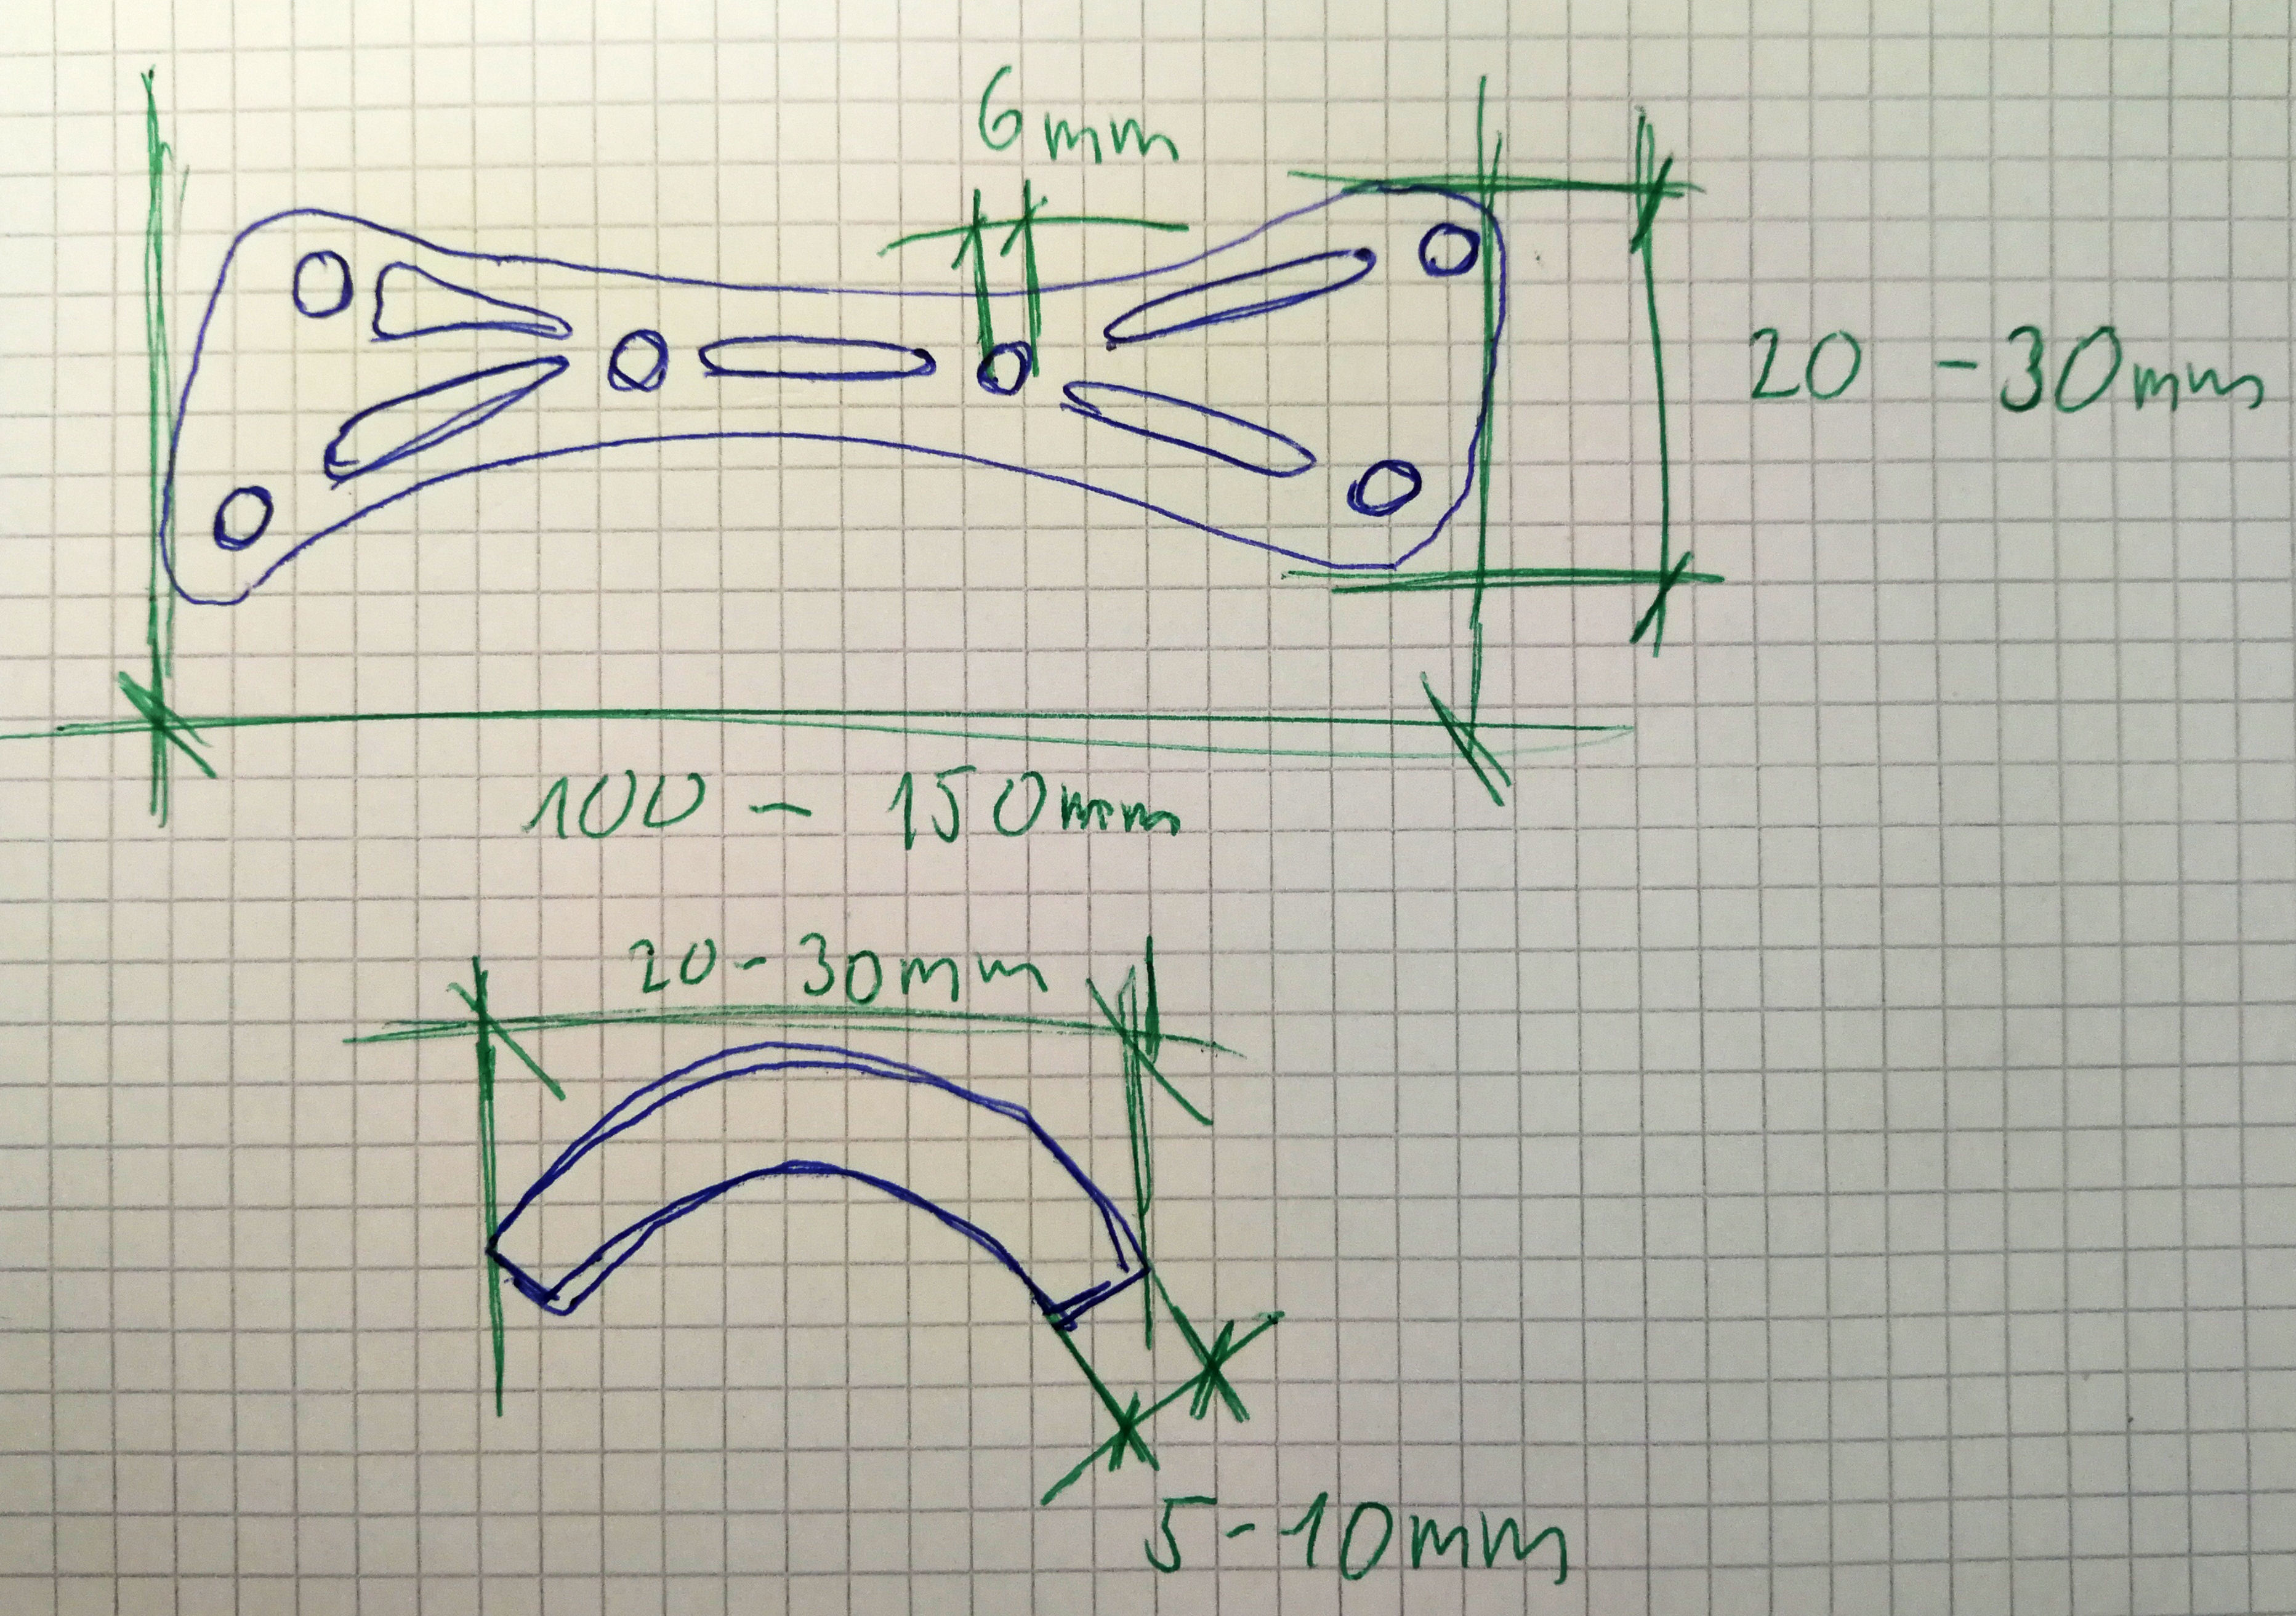
\includegraphics[width=15cm]{content/images/skizze.jpg}
		\captionof{figure}{Skizze der neuen Osteosyntheseplatte}
		\label{fig:skizze}
	\end{Figure}

\section{CAD Modellierung}

	In \textit{CATIA V5} wurden zwei Platten entworfen. Die erste Platte (Abb. \ref{fig:drawing_compare}) ist
	sehr einfach gehalten. Diese wird als Vergleich zu der weiterentwickelten Platte (Abb. \ref{fig:drawing_osp})
	benutzt.
	
	Es können nur winkelstabile Schrauben benutzt werden. Kompression geht in diesen Öffnungen nicht.

	\subsection{Zeichnungen}
	
		\subsubsection{Vergleichsplatte}
			\begin{Figure}
				\centering
				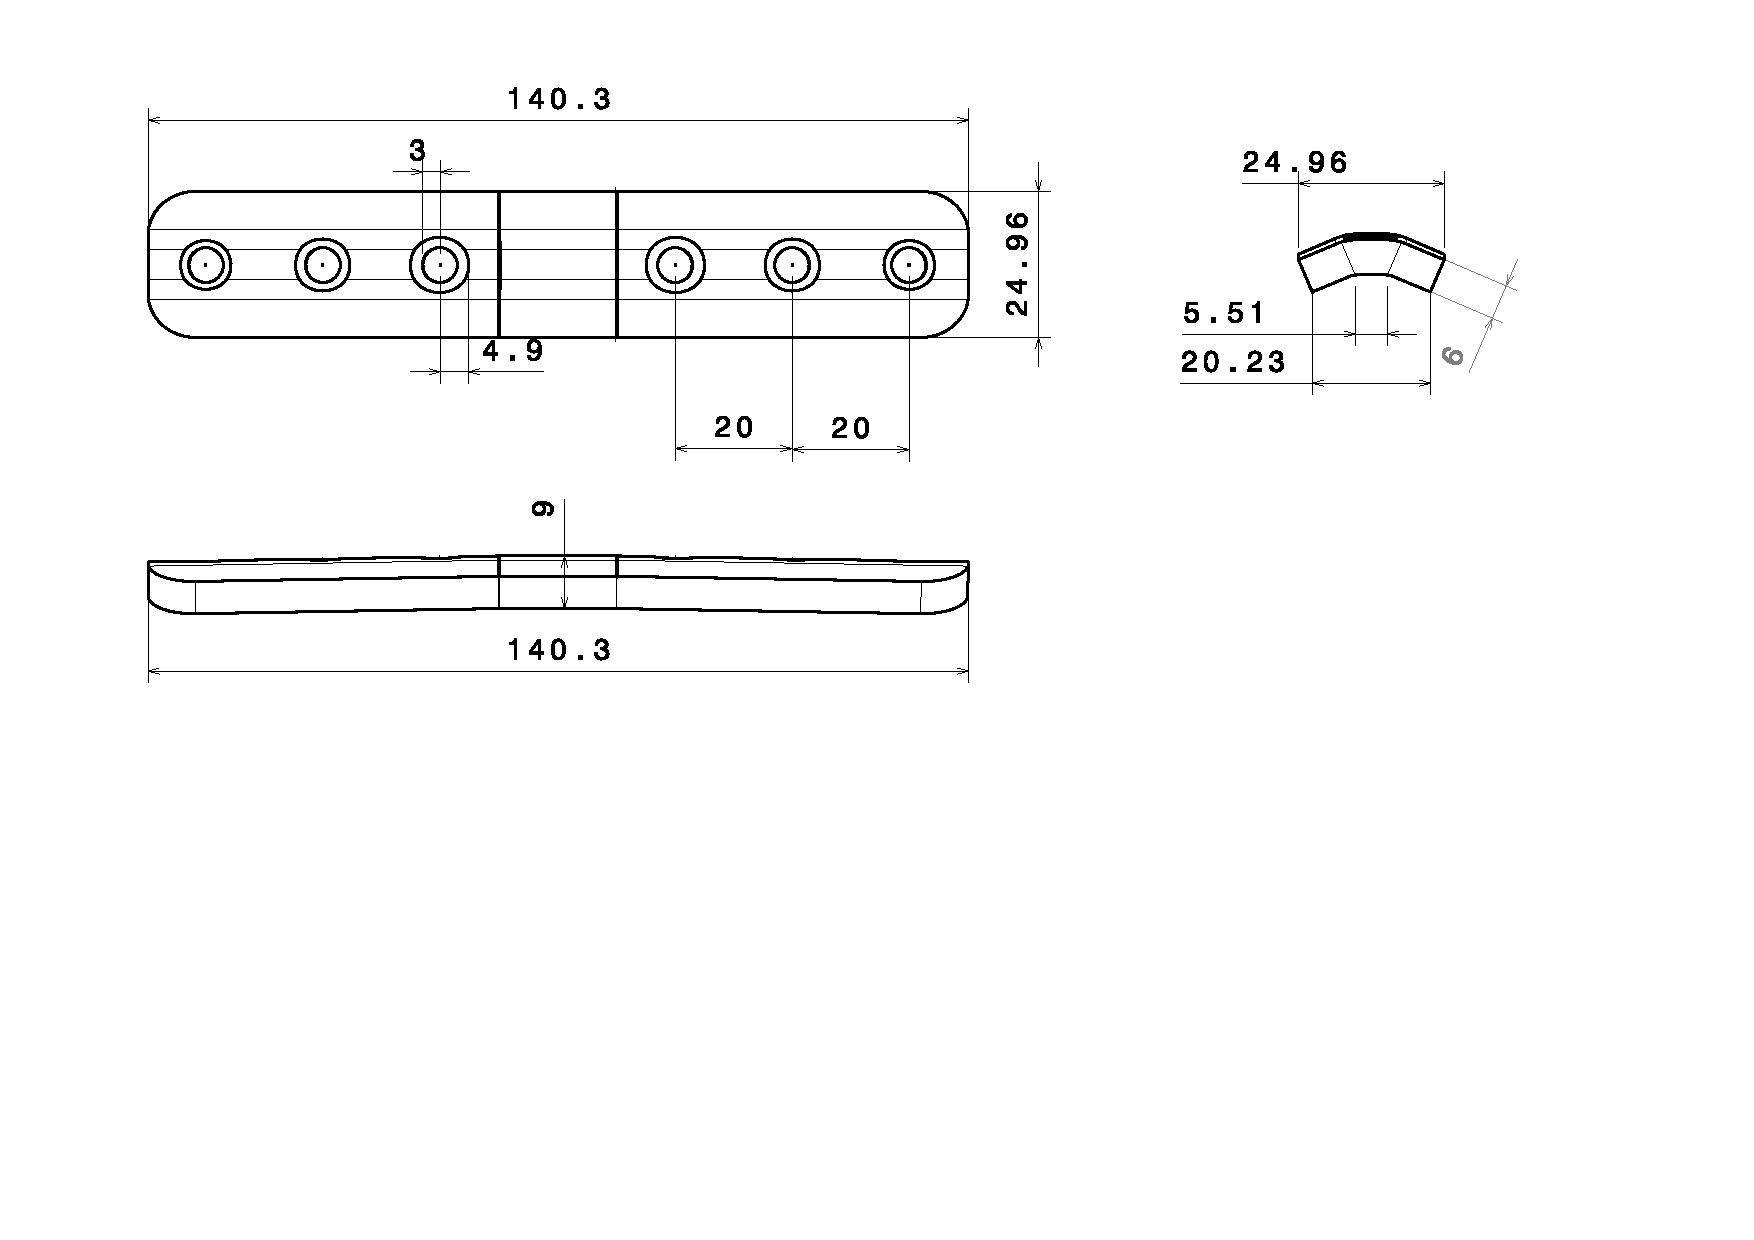
\includegraphics[trim={1.5cm 8.5cm 3.5cm 0.5cm},clip,width=15cm]{content/drawing_compare.pdf}
				\captionof{figure}{Vergleichsplatte}
				\label{fig:drawing_compare}
			\end{Figure}
		
		\subsubsection{Erweiterte Platte}
			\begin{Figure}
				\centering
				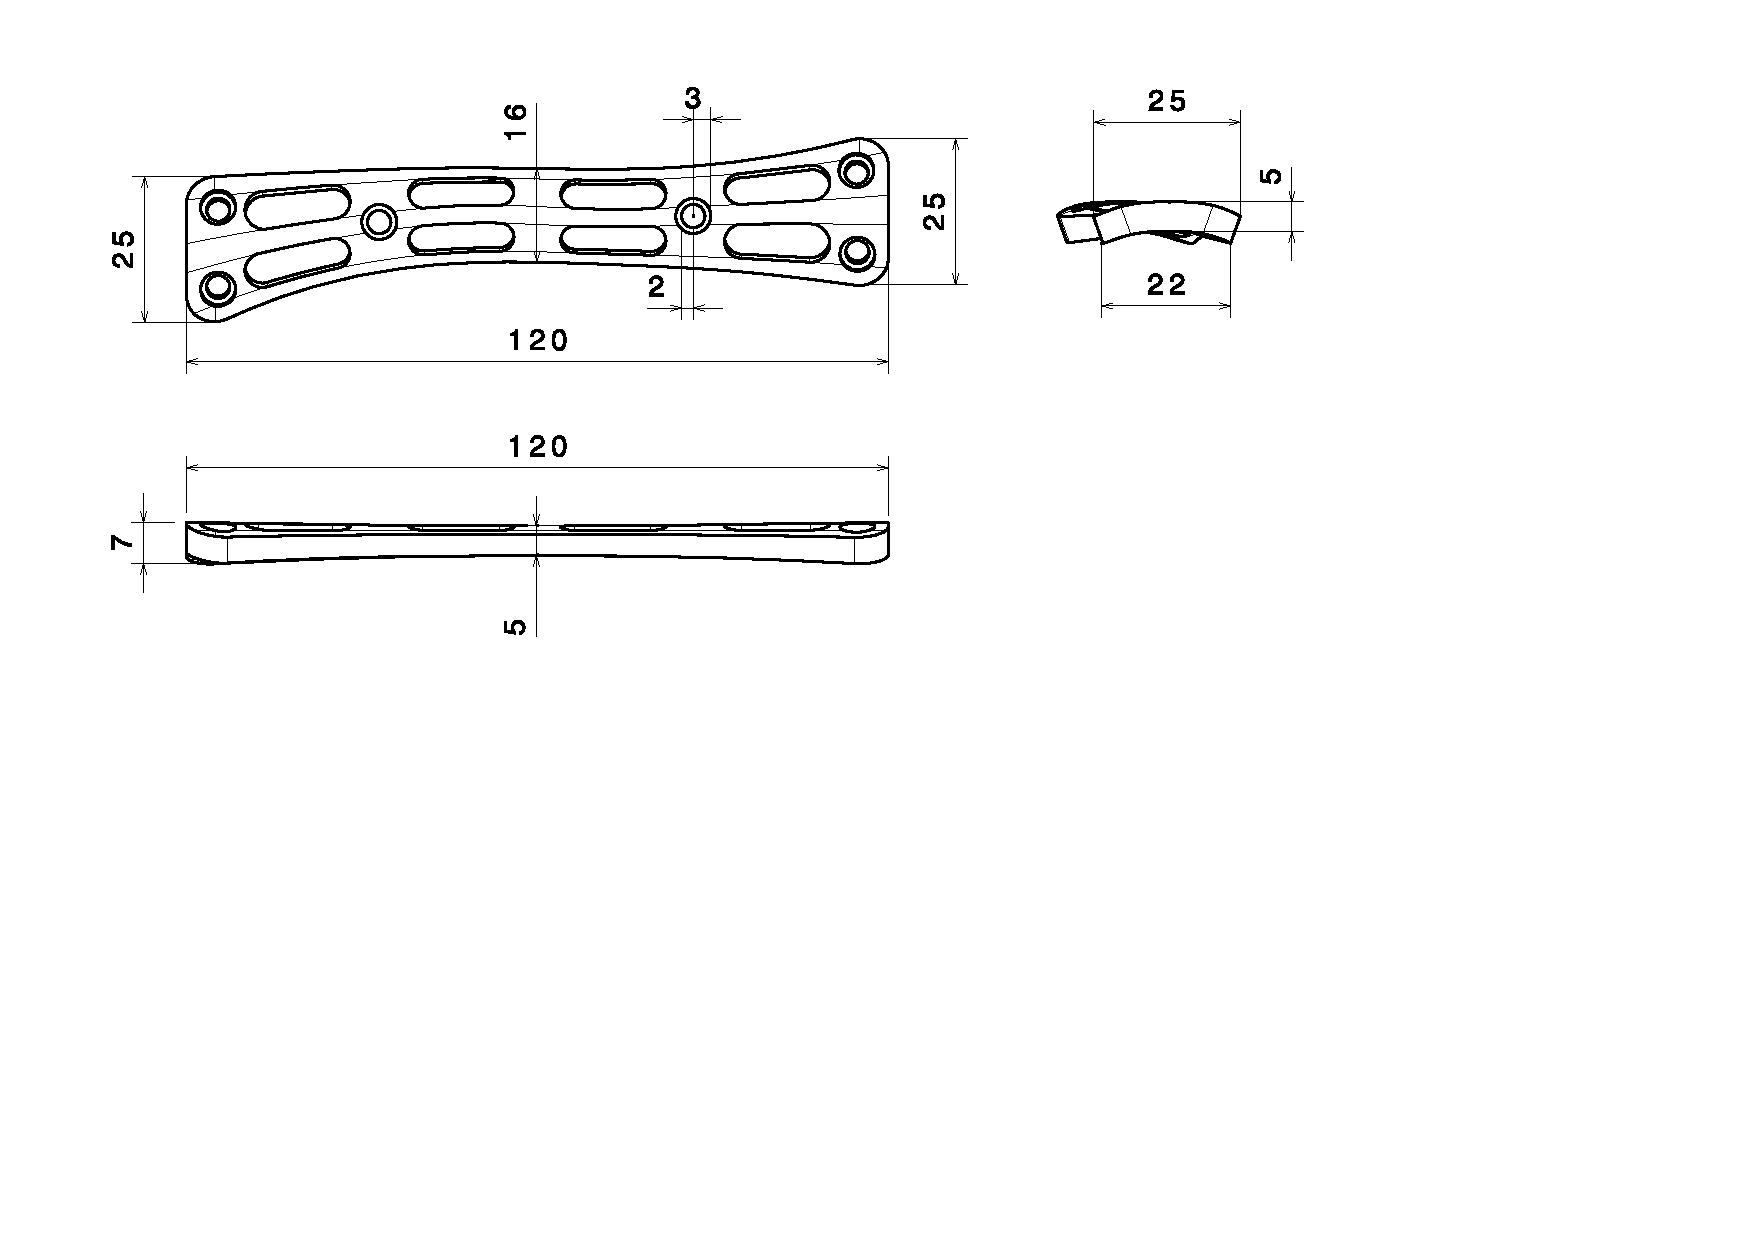
\includegraphics[trim={1.5cm 10cm 7cm 0.5cm},clip,width=15cm]{content/drawing_osp.pdf}
				\captionof{figure}{Erweiterte Platte}
				\label{fig:drawing_osp}
			\end{Figure}

	\subsection{Rendering}
		\begin{Figure}
			\centering
			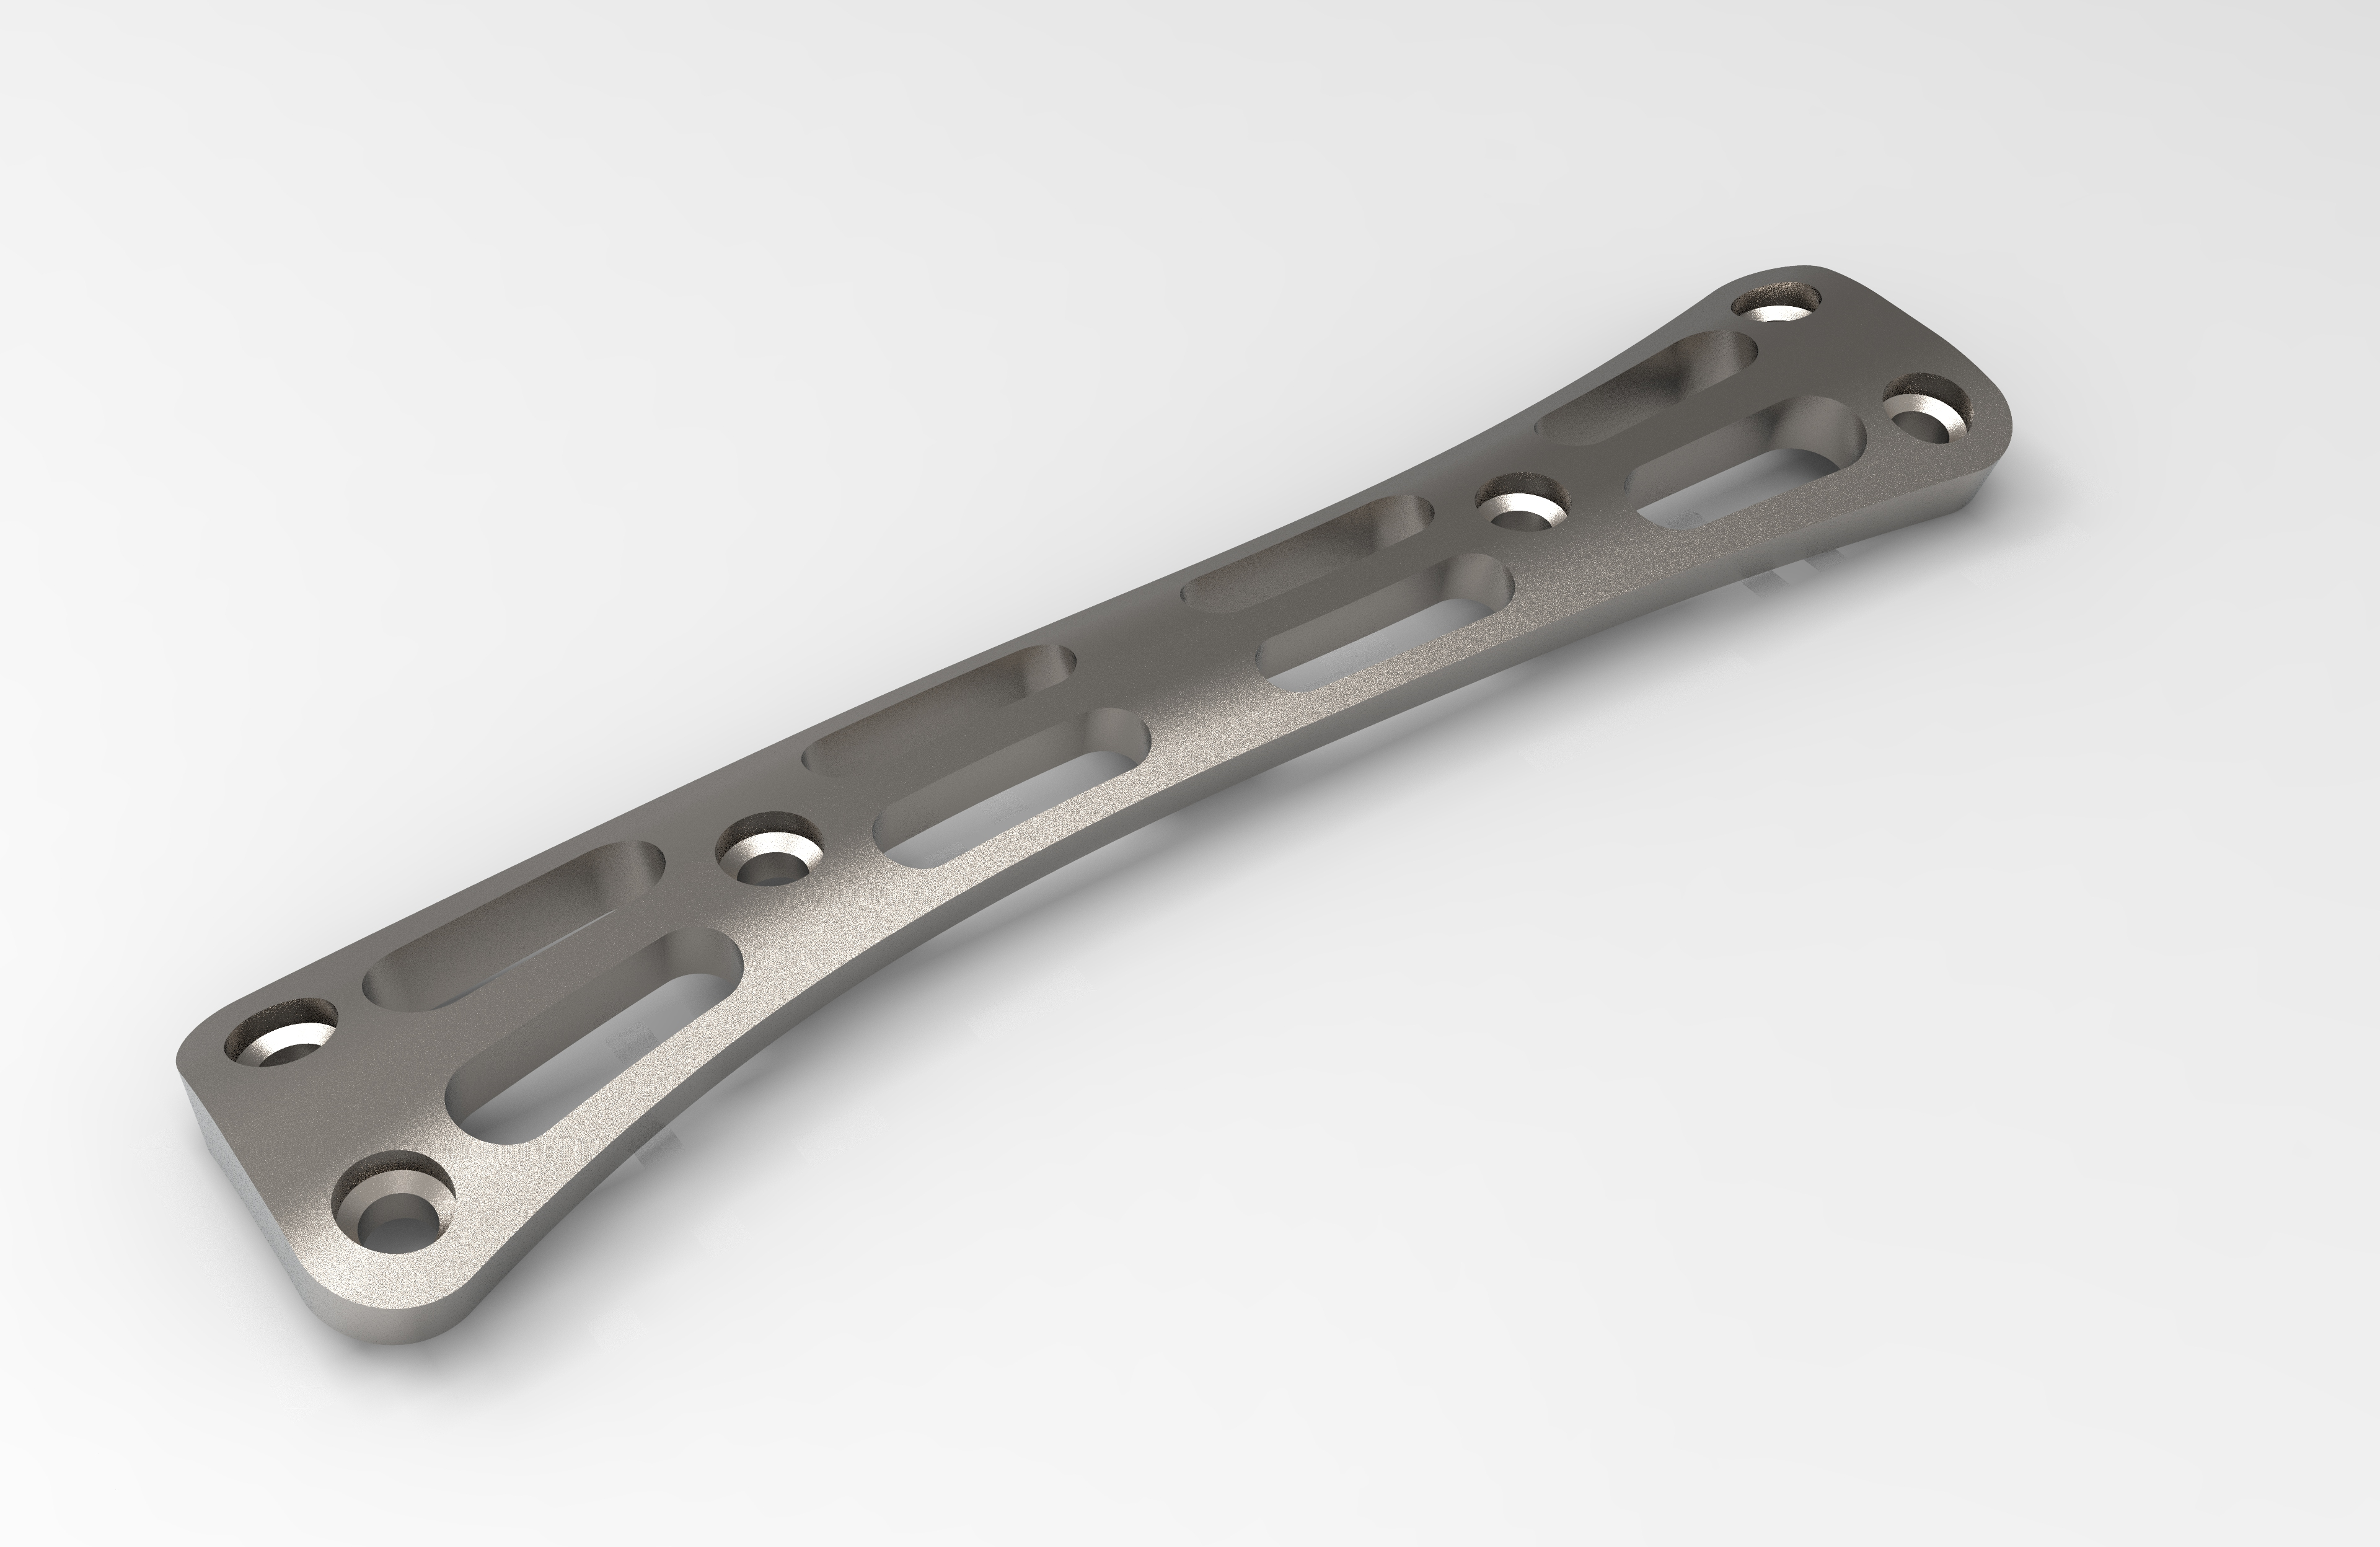
\includegraphics[width=15cm]{content/images/rendering.jpg}
			\captionof{figure}{Osteosyntheseplatte ohne Schrauben}
			\label{fig:rendering}
		\end{Figure}
	
		\begin{Figure}
			\centering
			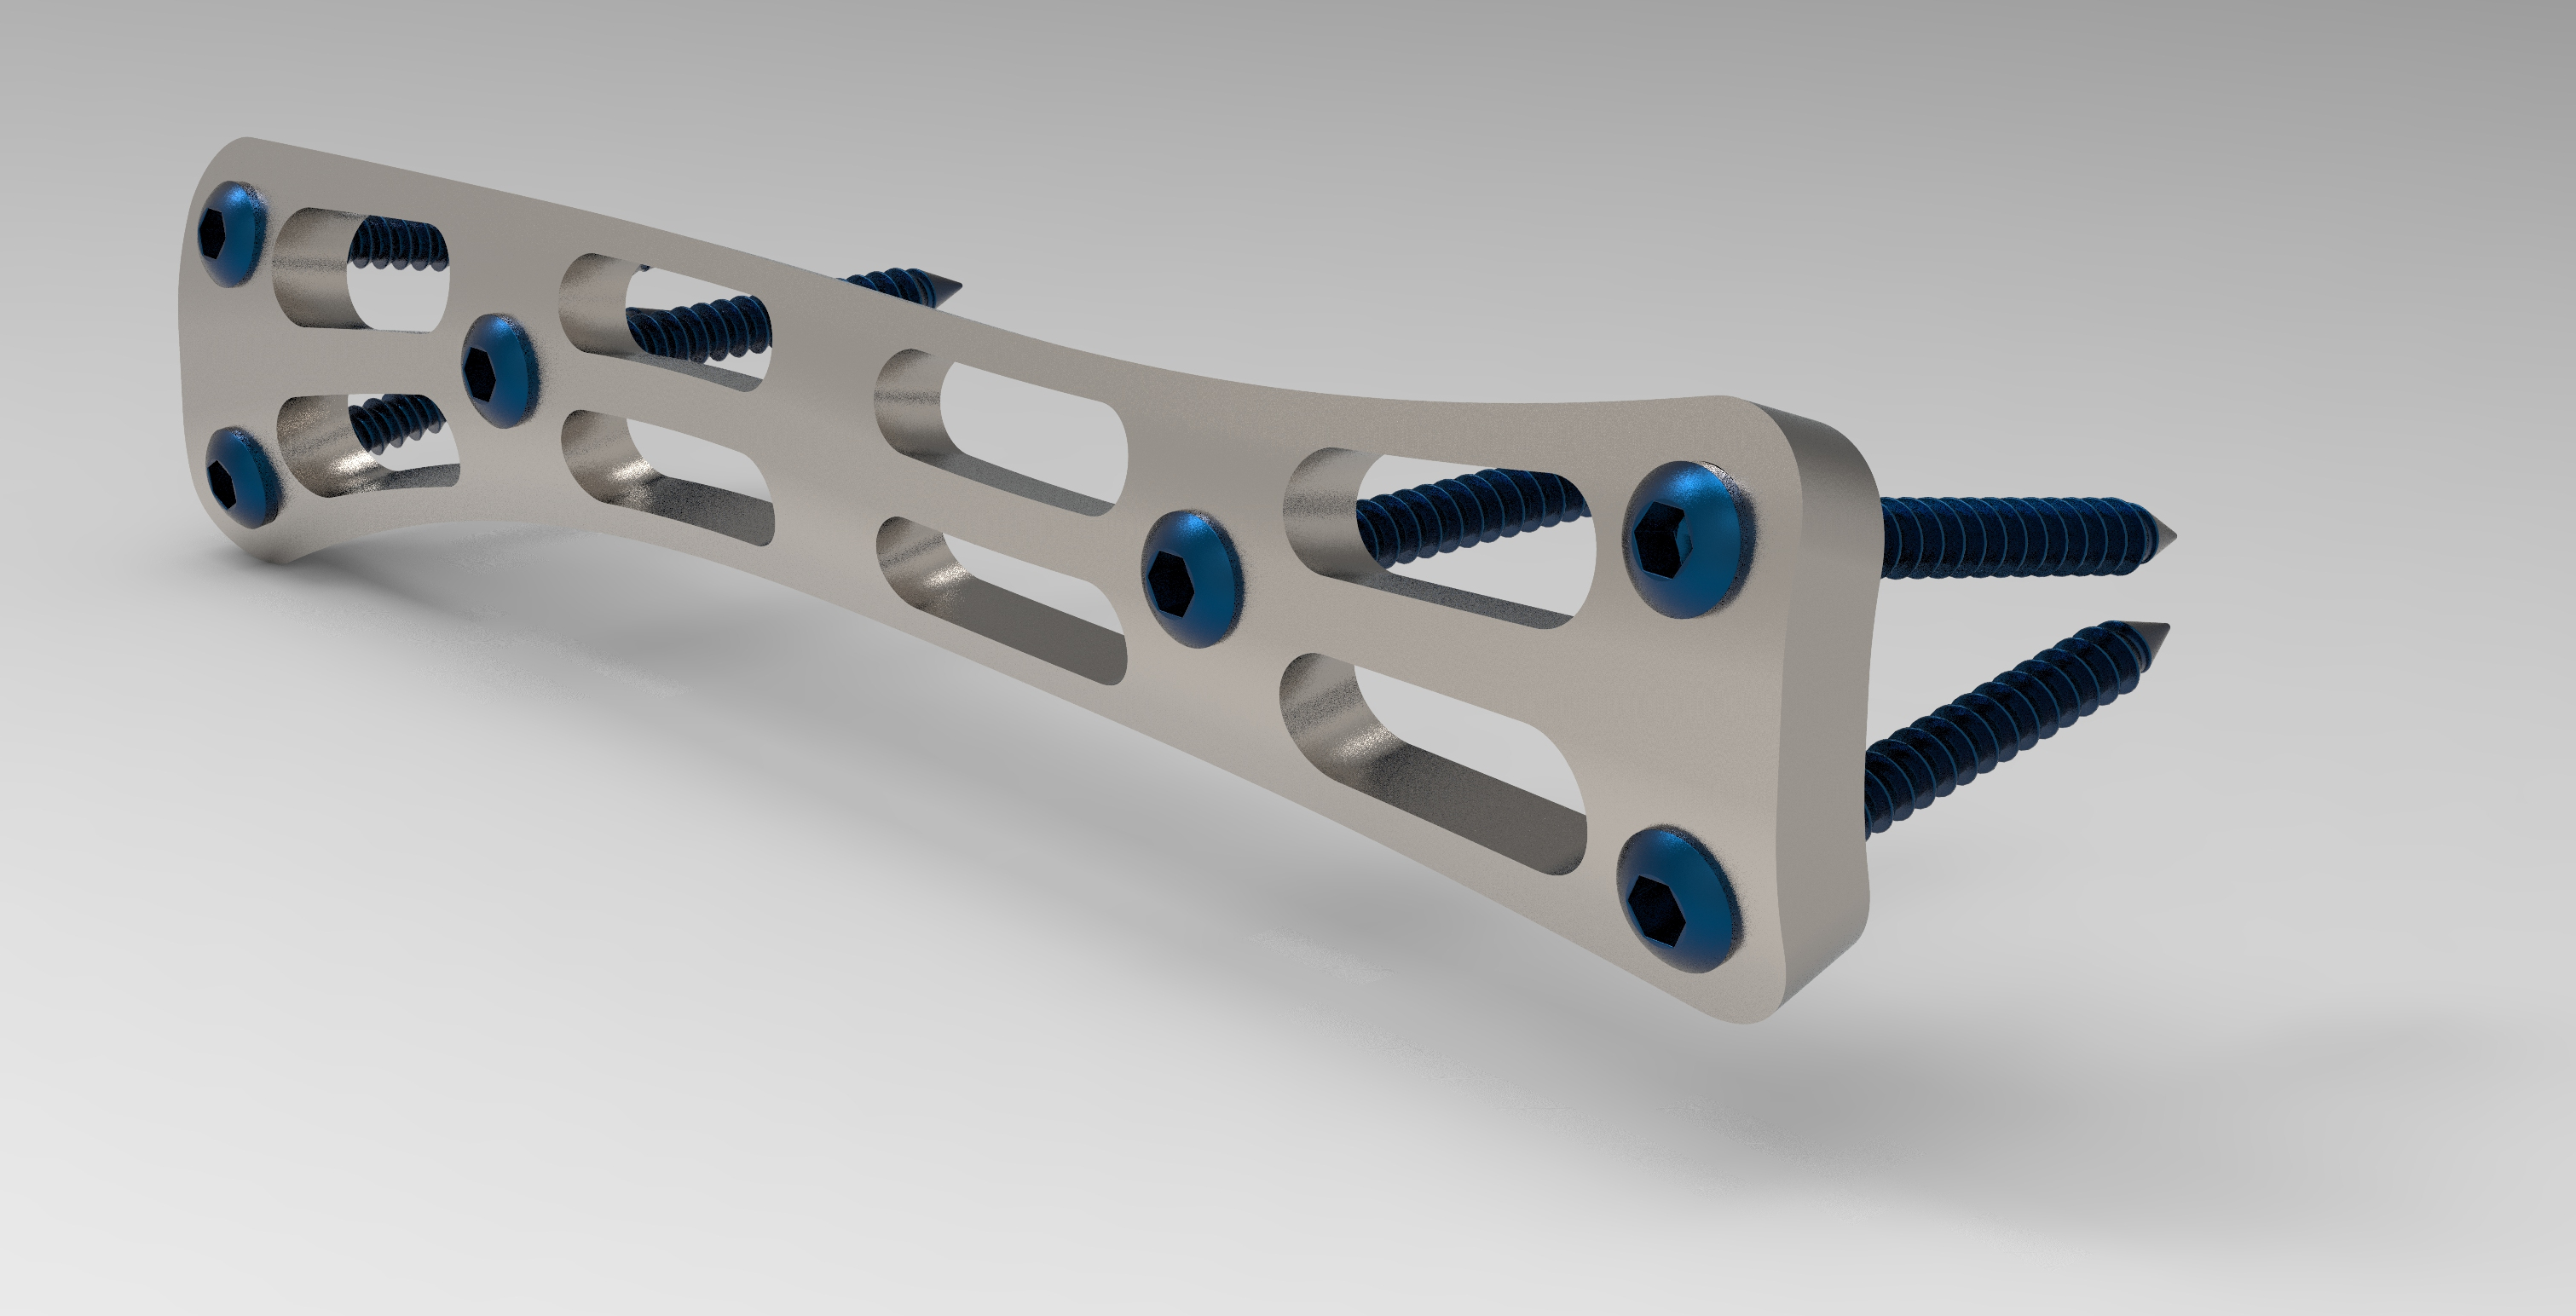
\includegraphics[width=15cm]{content/images/rendering_screws.jpg}
			\captionof{figure}{Osteosyntheseplatte mit Schrauben}
			\label{fig:rendering_screws}
		\end{Figure}
			
		\begin{Figure}
			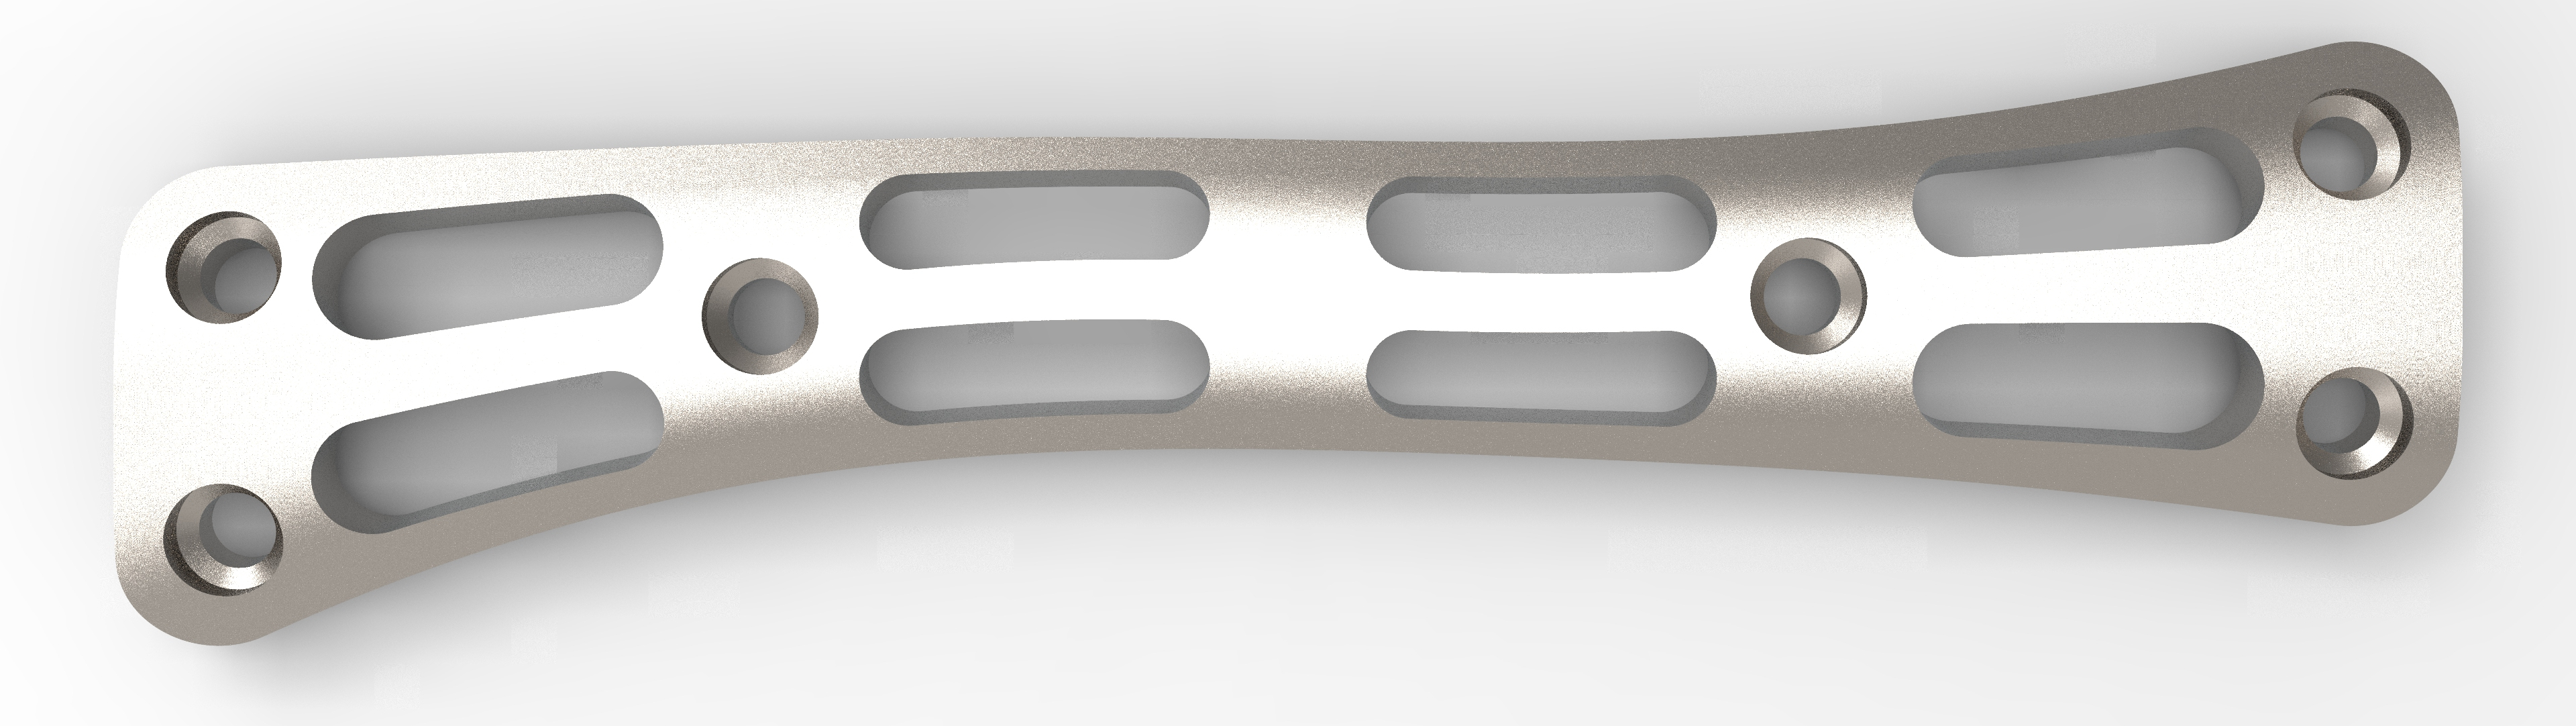
\includegraphics[width=15cm]{content/images/rendering_top.jpg}
			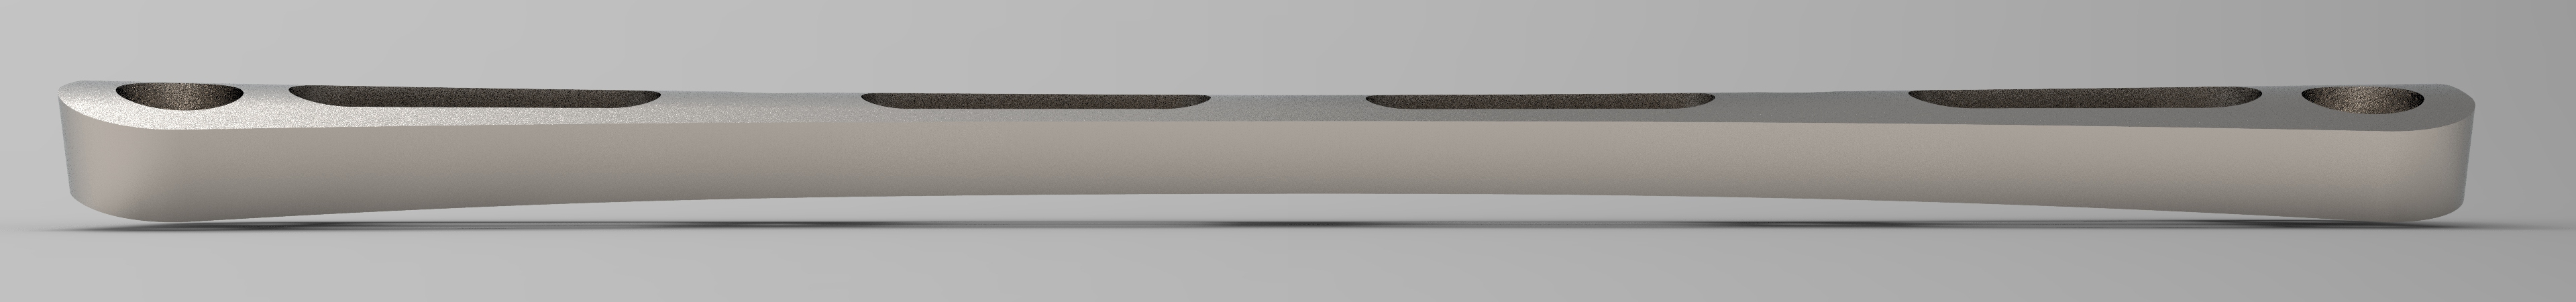
\includegraphics[width=15cm]{content/images/rendering_side.jpg}
			
\includegraphics[width=15cm]{content/images/rendering_front.jpg}
			\captionof{figure}{Osteosyntheseplatte (oben, seite, vorne)}
			\label{fig:rendering_side}
		\end{Figure}

\newpage
\section{FEM Analyse}

	In \textit{Ansys Workbench} wurde nun eine statische FE-Analyse durchgeführt.
	
	\subsection{Materialdaten}
		\begin{center}
			\renewcommand{\arraystretch}{1.5}
			\begin{tabular}{ | p{6cm} | p{3cm} | p{3cm} | }
				\multicolumn{1}{l}{\bfseries Material} &
				\multicolumn{1}{l}{\bfseries Dichte} &
				\multicolumn{1}{l}{\bfseries E-Modul } \\ \hline
				
				Knochen (bone) & \SI{1300}{\frac{kg}{m^3}} & \SI{17}{GPa} \\ \hline
				Titanlegierung (titanium alloy) & \SI{4620}{\frac{kg}{m^3}} & \SI{96}{GPa} \\ \hline
			\end{tabular}
			\captionof{table}{Materialdaten}
			\label{tab:materials}
		\end{center}

	\subsection{Vernetzung}
		\begin{Figure}
			\centering
			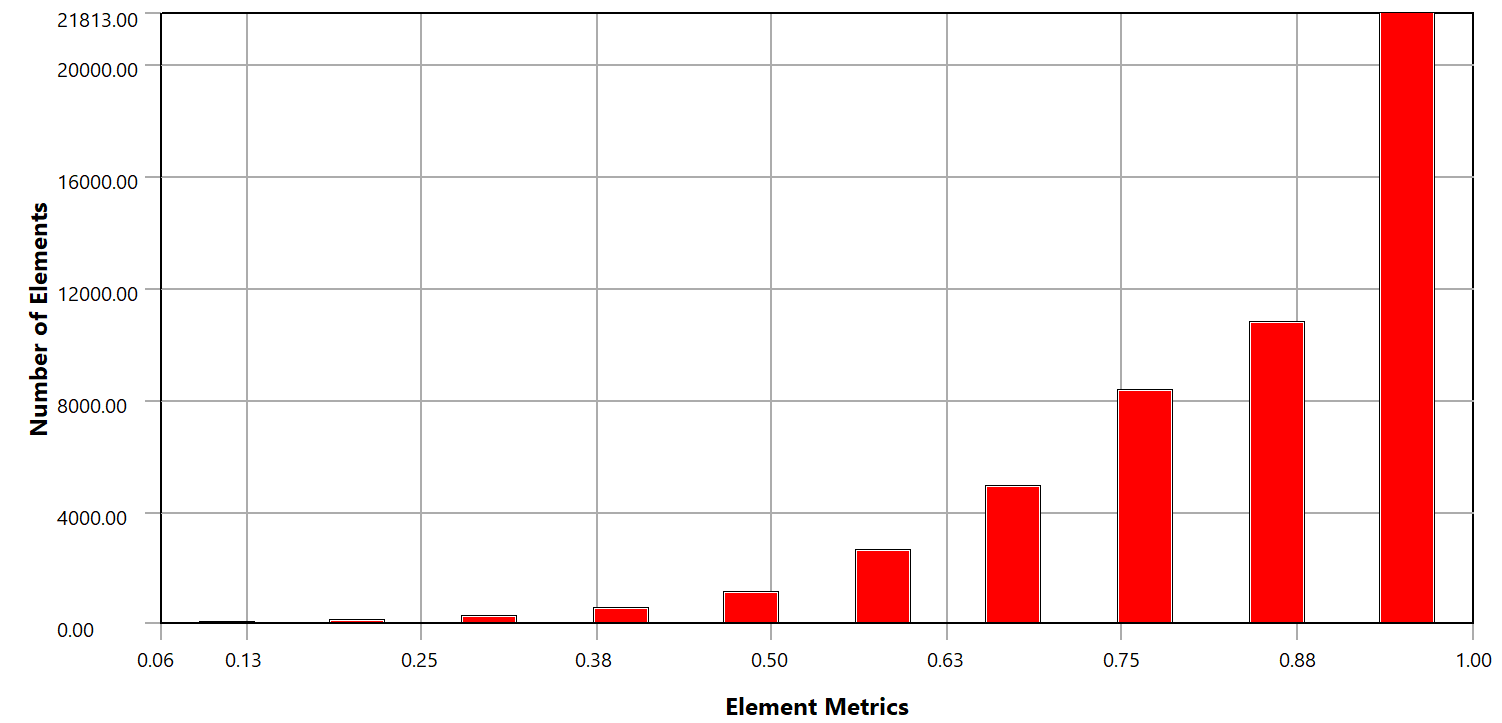
\includegraphics[width=15cm]{content/images/mesh_quality.png}
			\captionof{figure}{Element Qualität des Meshes. Der grosste Teil der Elemente
				               haben eine gute oder sogar sehr gute Qualität}
			\label{fig:mesh_quality}
		\end{Figure}
		
		\begin{Figure}
			\centering
			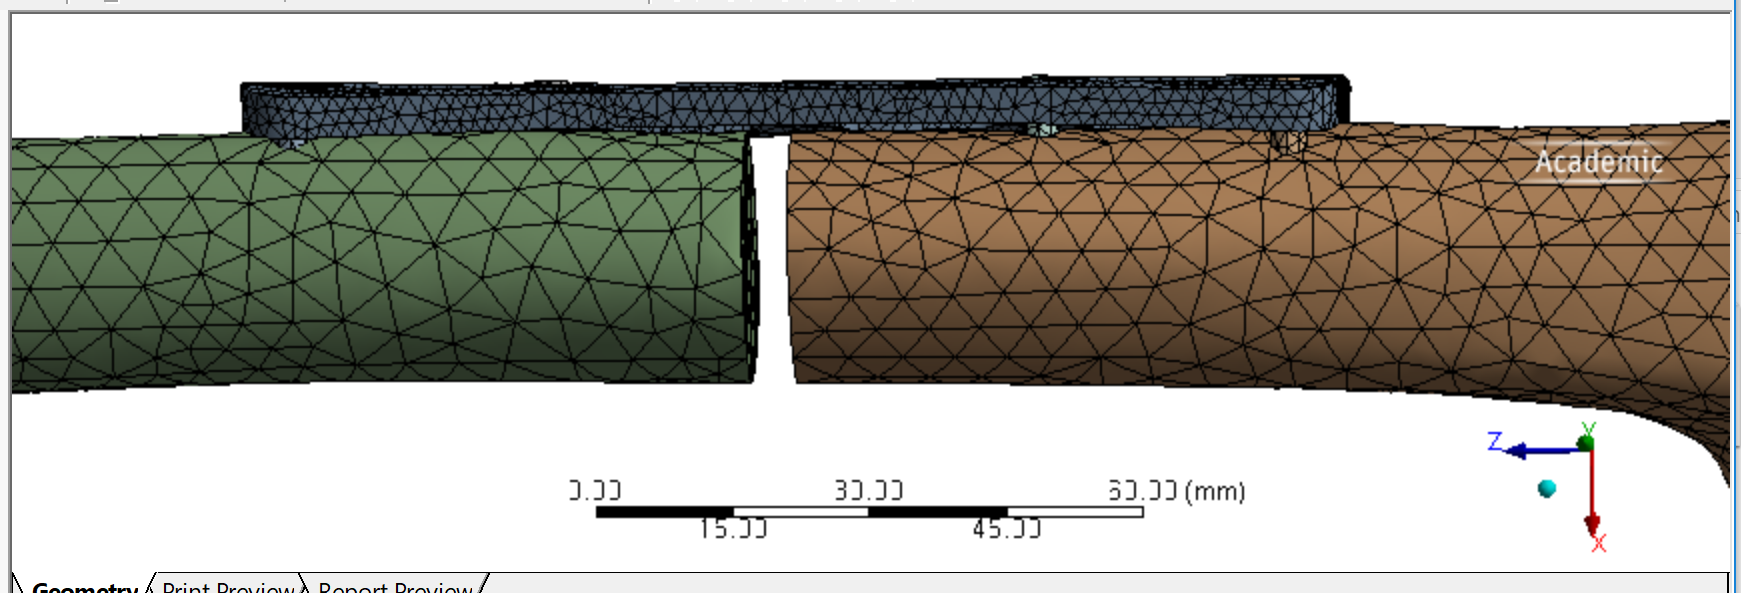
\includegraphics[width=15cm]{content/images/mesh_quality_graph_2.png}
			\captionof{figure}{Meshing von der Seite}
			\label{fig:device3}
		\end{Figure}
		
		\begin{Figure}
			\centering
			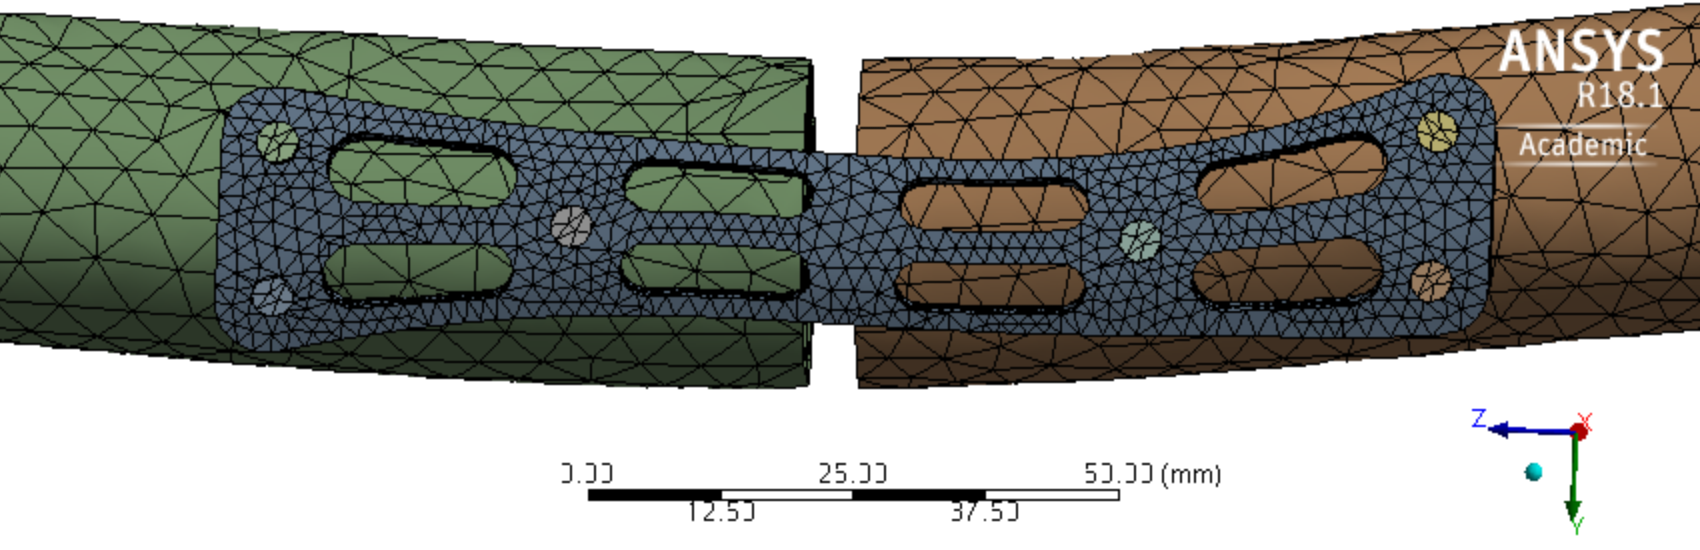
\includegraphics[width=15cm]{content/images/mesh_quality_graph_3.png}
			\captionof{figure}{Meshing von oben}
			\label{fig:device3}
		\end{Figure}

	\subsection{Kräfte}
	
		Die Gelenkwinkel, Muskel- und Reaktionskräfte wurden letztes Semester in einer
		Bewegungsanalyse erhoben. Die Probandin ist Stephanie Ruch. Mit \textit{OpenSim} wurden
		die Daten graphisch aufbereitet. Der Zeitpunkt, an dem die maximale Kraft aufgebracht
		wurde ist $ t_0 = \SI{2.2}{s} $.
		
		\begin{mycapequ}[!ht]
			\vspace{-5mm}
			\begin{align*}
				t_0 = \SI{2.2}{s}
			\end{align*}
			\vspace{-8mm}
		\end{mycapequ}
	
		\begin{Figure}
			\centering
			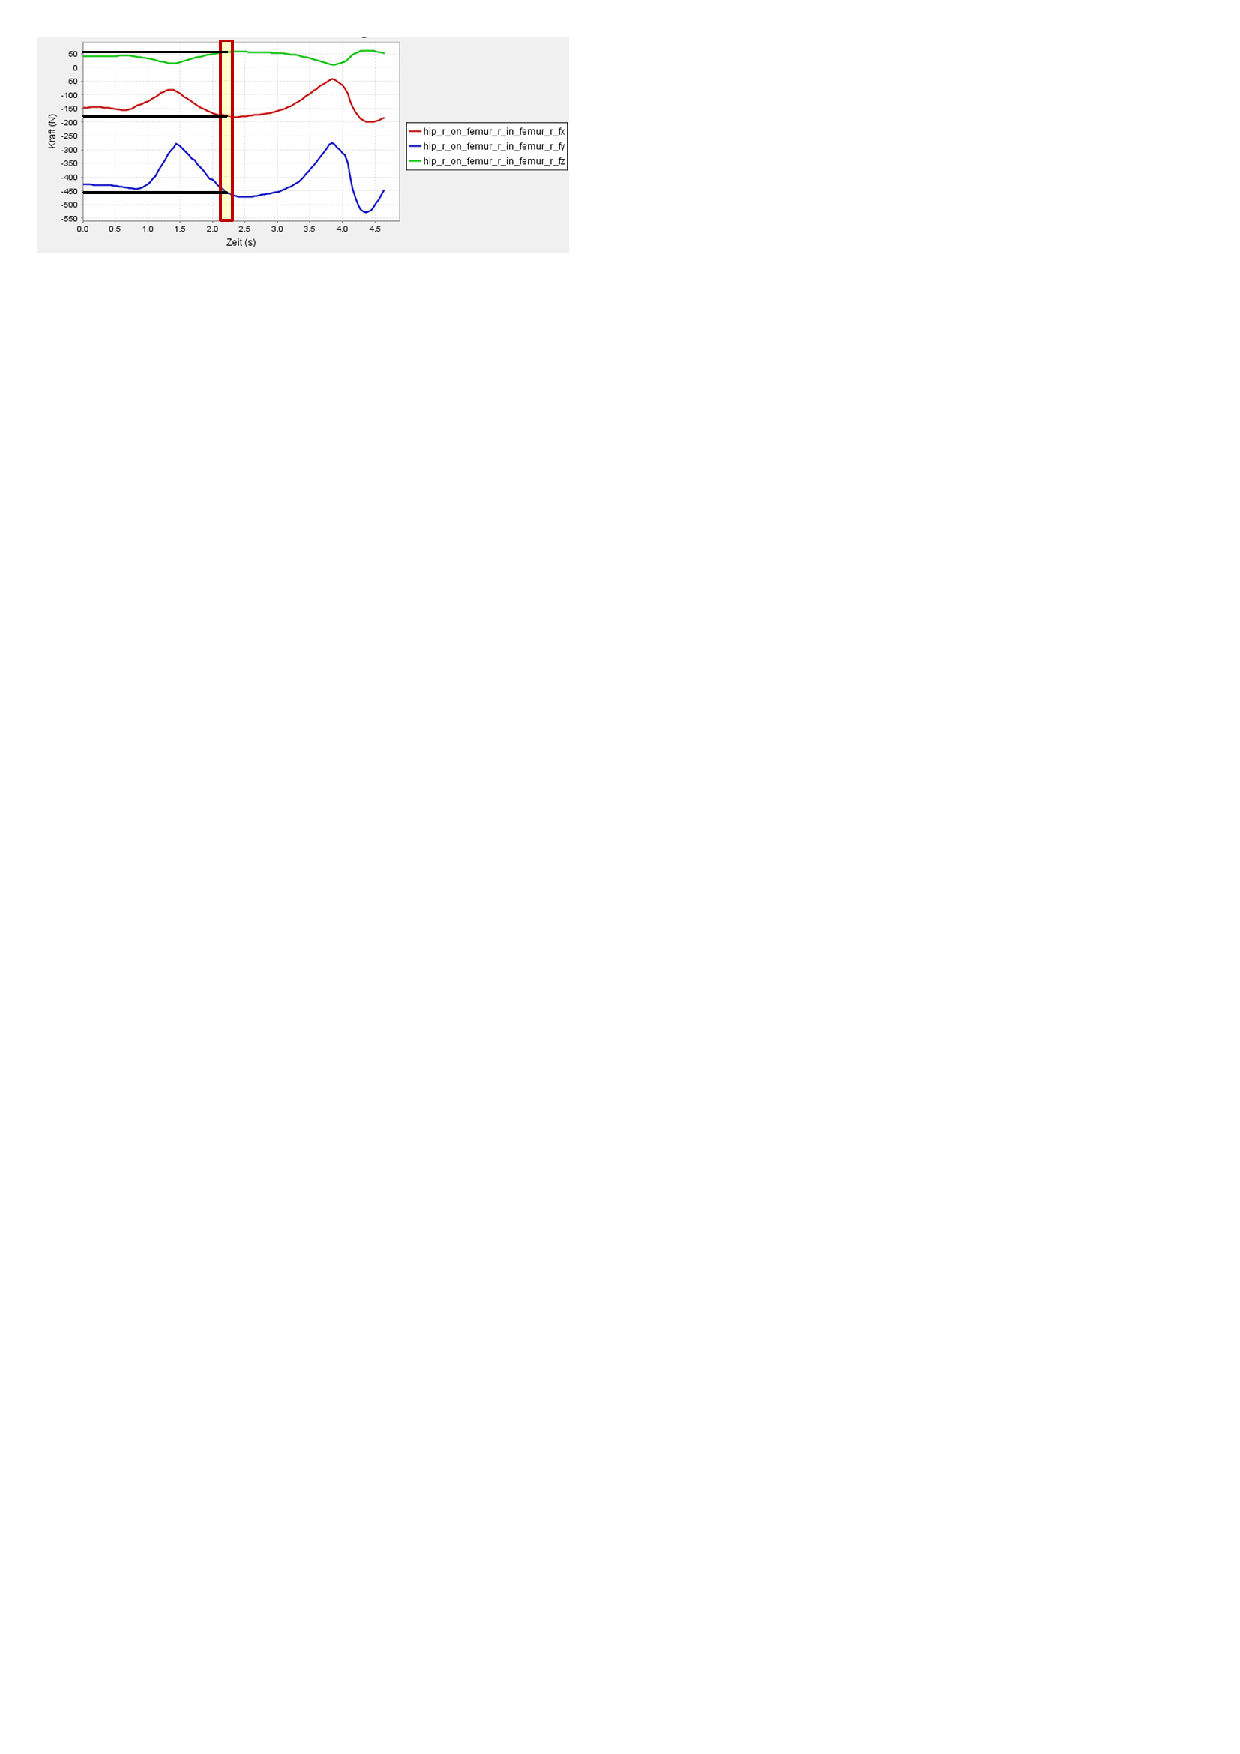
\includegraphics[trim={0.5cm 25.25cm 11.25cm 0.5cm},clip,width=12cm]{content/opensim_hip_reaction_force.pdf}
			\captionof{figure}{OpenSim Reaktionskräfte am Femur}
			\label{fig:excel}
		\end{Figure}
	
		\begin{Figure}
			\centering
			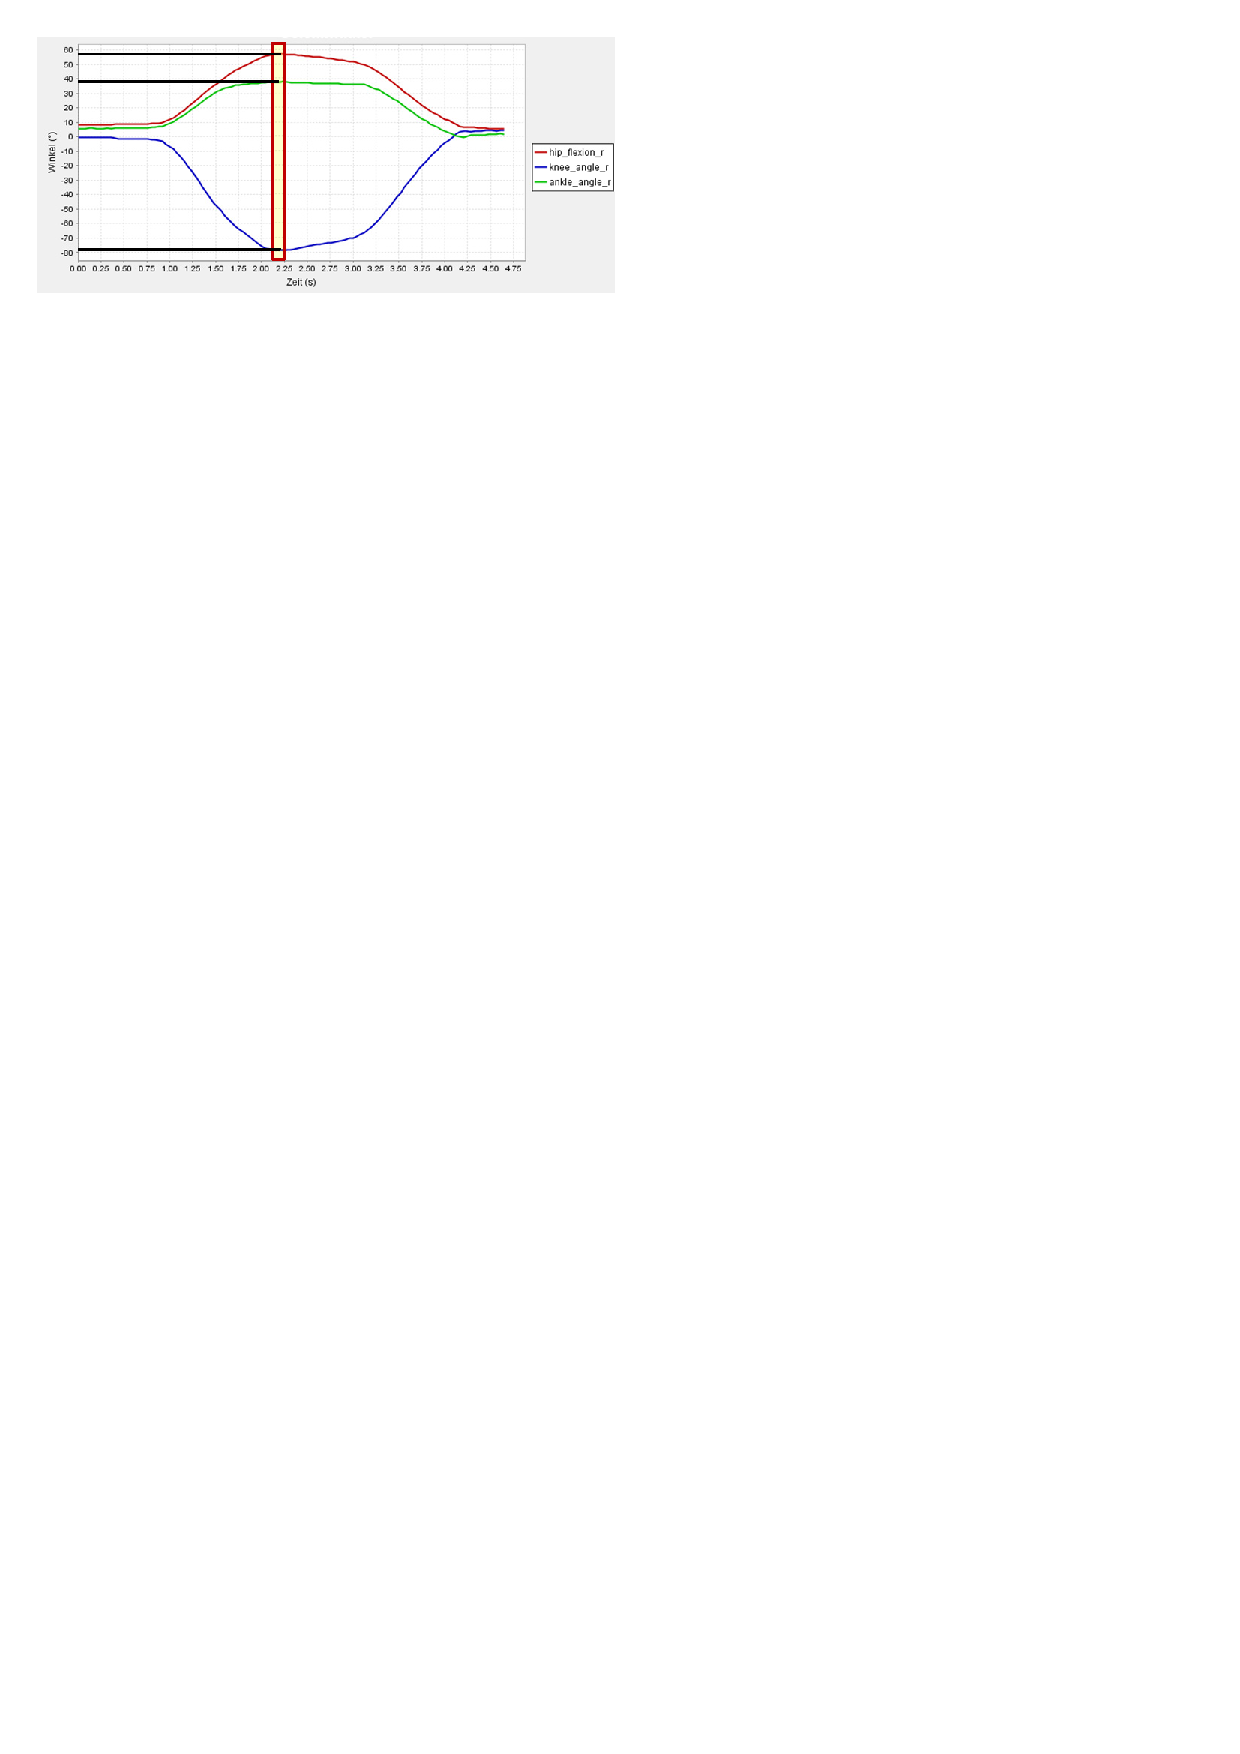
\includegraphics[trim={0.5cm 24.25cm 10.5cm 0.5cm},clip,width=12cm]{content/opensim_joint_angles.pdf}
			\captionof{figure}{OpenSim Gelenkwinkel}
			\label{fig:excel}
		\end{Figure}
		
		\begin{Figure}
			\centering
			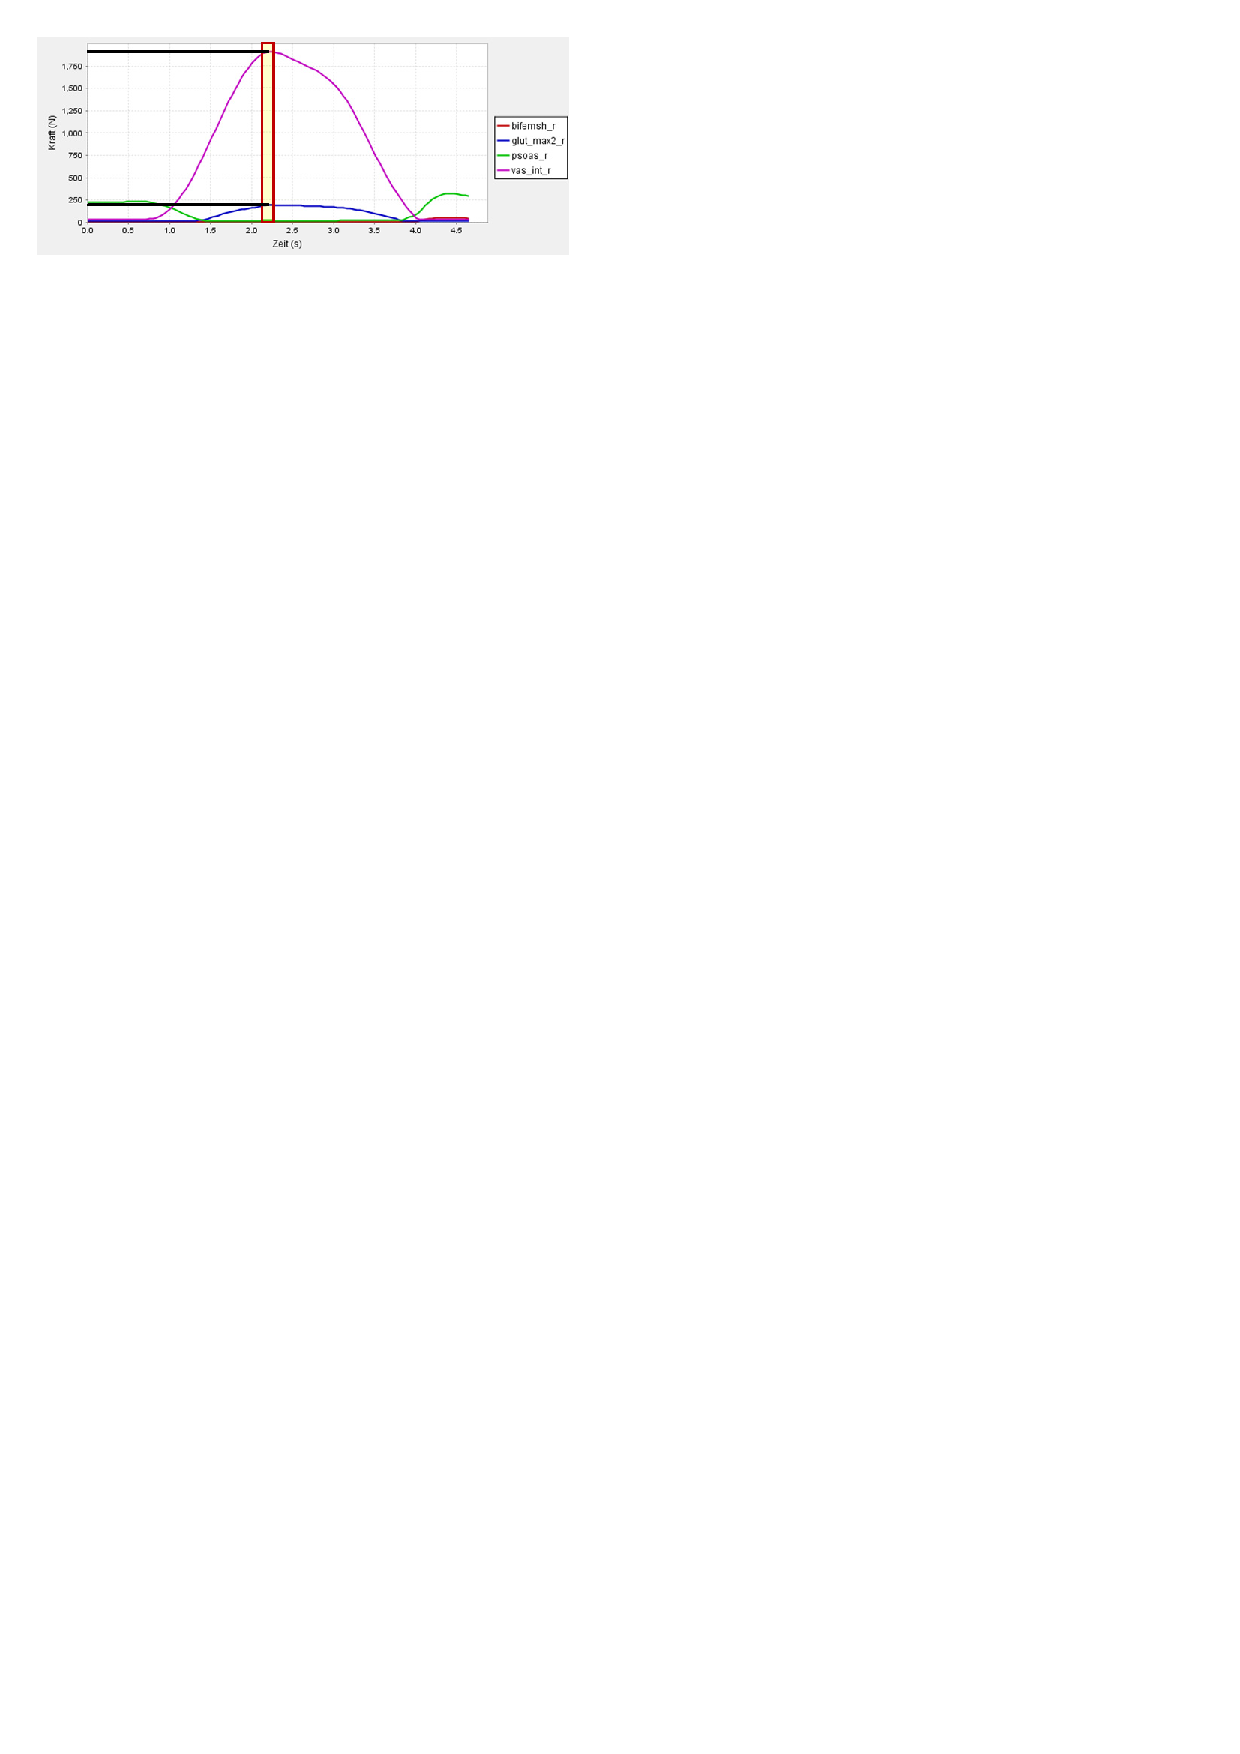
\includegraphics[trim={0.5cm 25.25cm 11.25cm 0.5cm},clip,width=12cm]{content/opensim_muscle_force.pdf}
			\captionof{figure}{OpenSim Muskelkräfte}
			\label{fig:excel}
		\end{Figure}
	
		\begin{Figure}
			\centering
			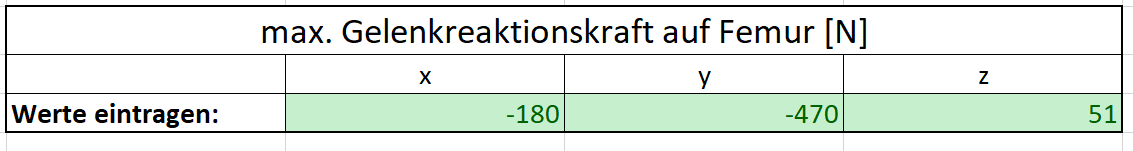
\includegraphics[width=15cm]{content/images/excel_1.png}
			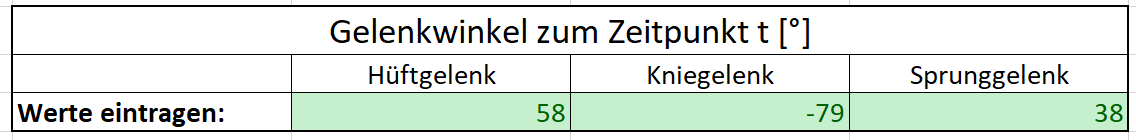
\includegraphics[width=15cm]{content/images/excel_2.png}
			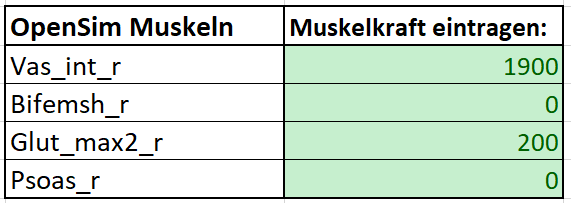
\includegraphics[width=8cm]{content/images/excel_3.png}
			\captionof{figure}{Gelenkreaktionskraft, Gelenkwinkel und Muskelkräfte}
			\label{fig:excel_1}
		\end{Figure}
	
		\begin{Figure}
			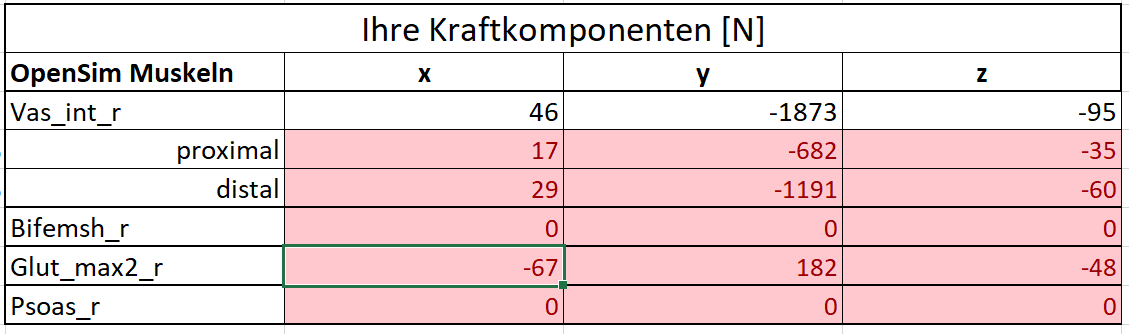
\includegraphics[width=15cm]{content/images/excel_4.png}
			\captionof{figure}{Von der vorherigen Abbildung wurde in Excel die Kraftkomponenten berechnet,
				               die dann in Ansys eingefügt wurden.}
			\label{fig:excel_4}
		\end{Figure}
	
		\begin{Figure}
			\centering
			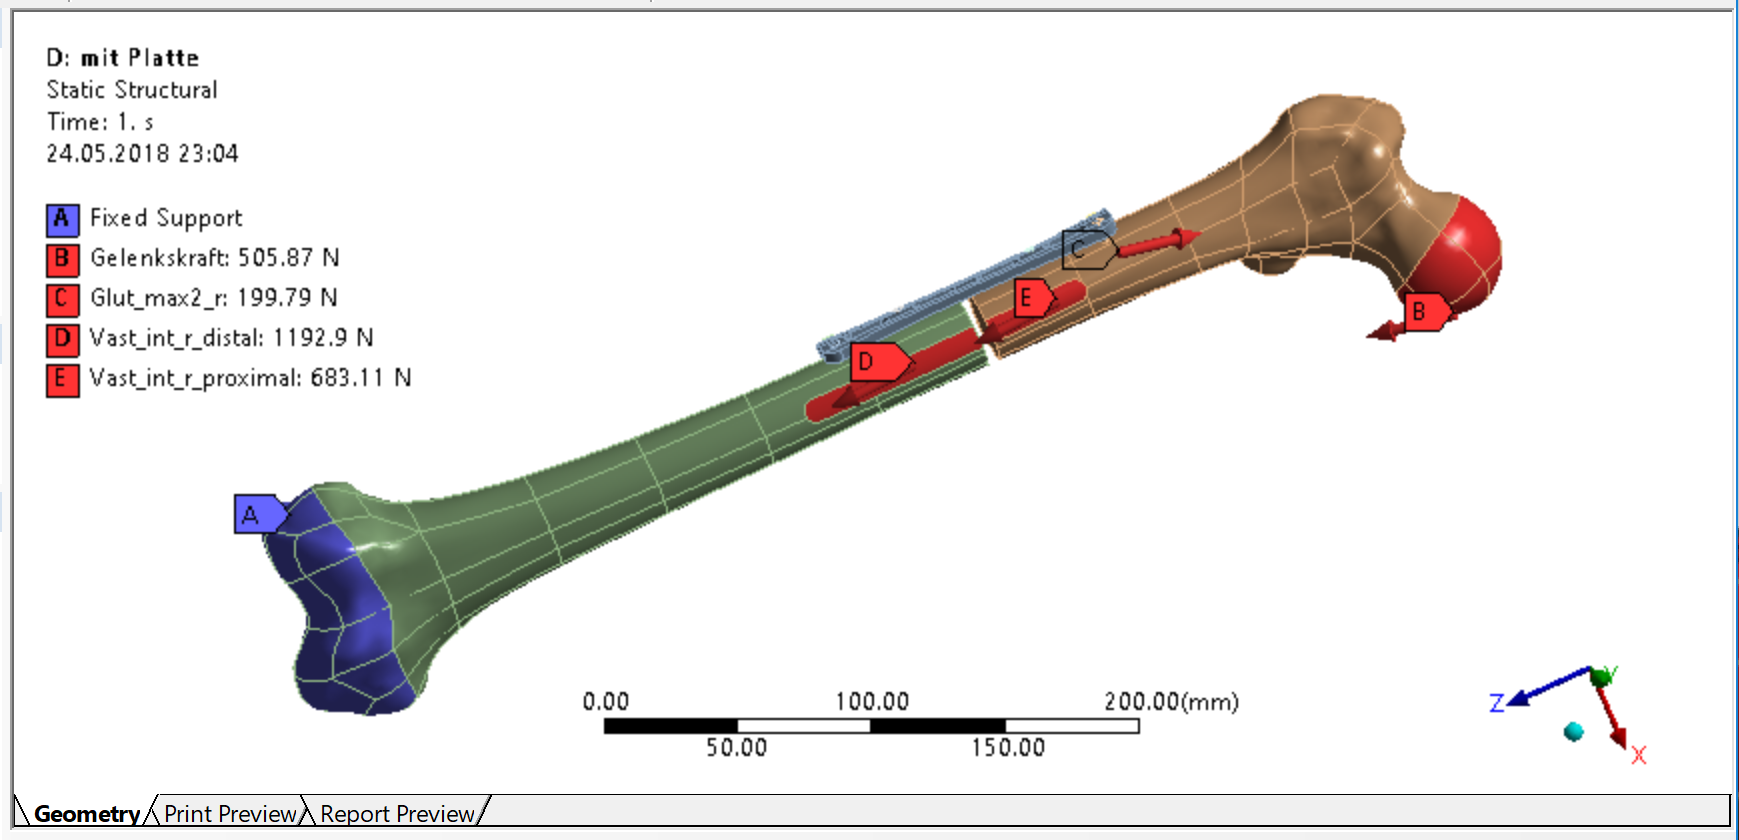
\includegraphics[width=15cm]{content/images/kraefte.png}
			\captionof{figure}{Fest eingespanntes Lager (blau), Muskel- und Gelenkkräfte (rot)}
			\label{fig:kraefte}
		\end{Figure}

\newpage
\section{Resultate}

	\subsection{Gesamtverformung}
	
		\begin{Figure}
			\centering
			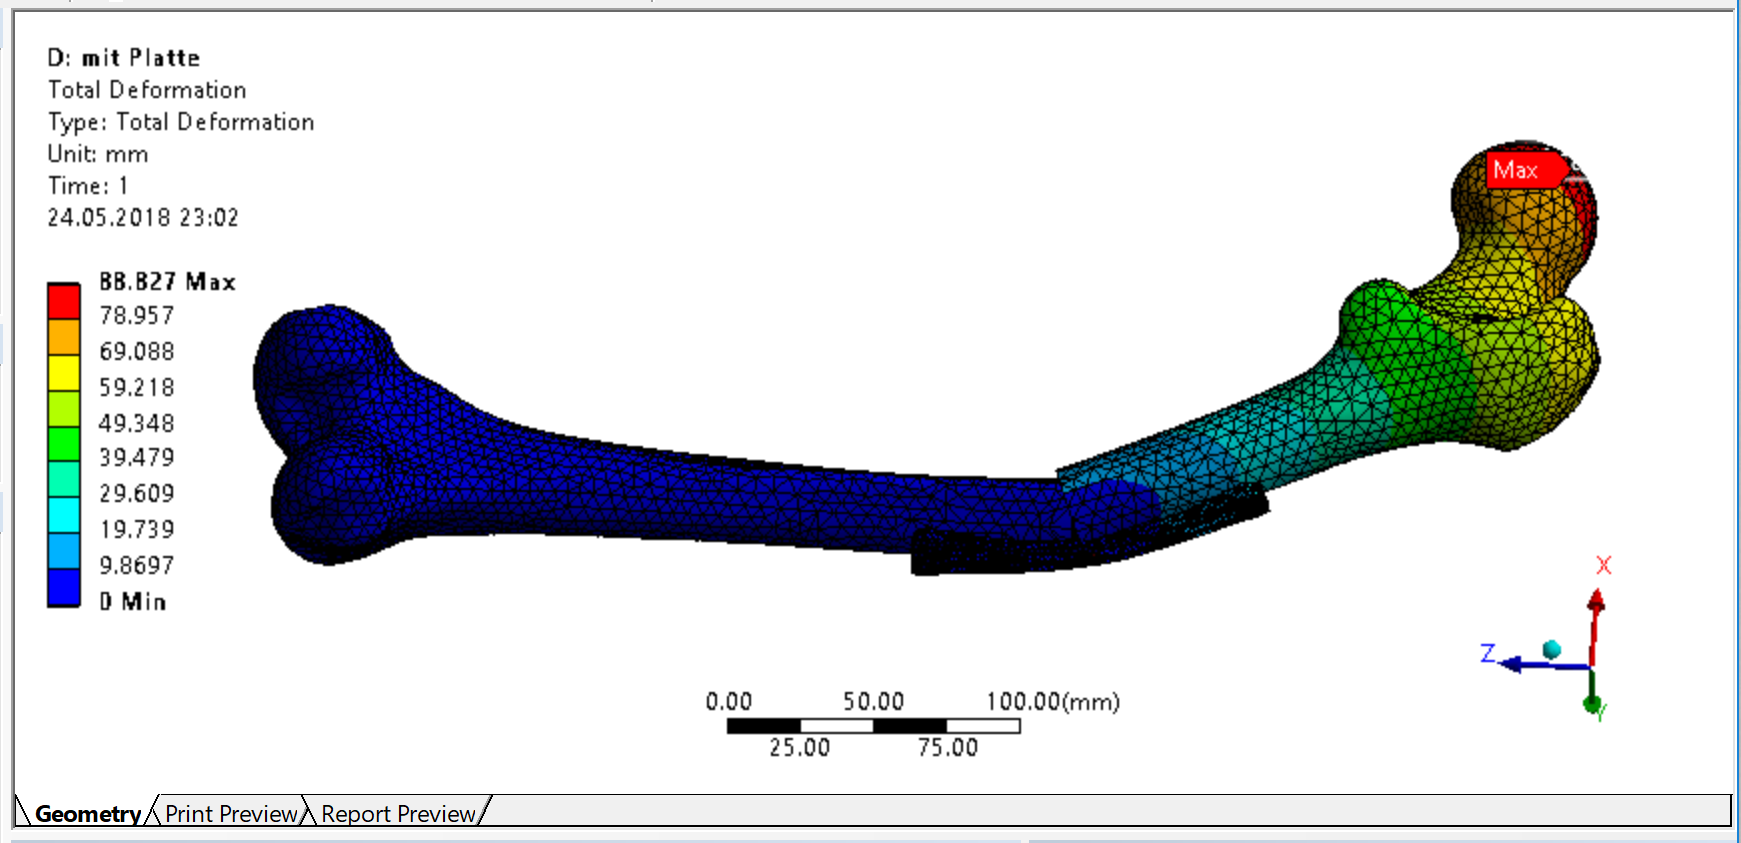
\includegraphics[width=15cm]{content/images/deformation.png}
			\captionof{figure}{Gesamtdeformation der Osteosyntheseplatte}
			\label{fig:deformation}
		\end{Figure}
	
		\subsubsection{Vergleichsplatte}
	
			\begin{Figure}
				\centering
				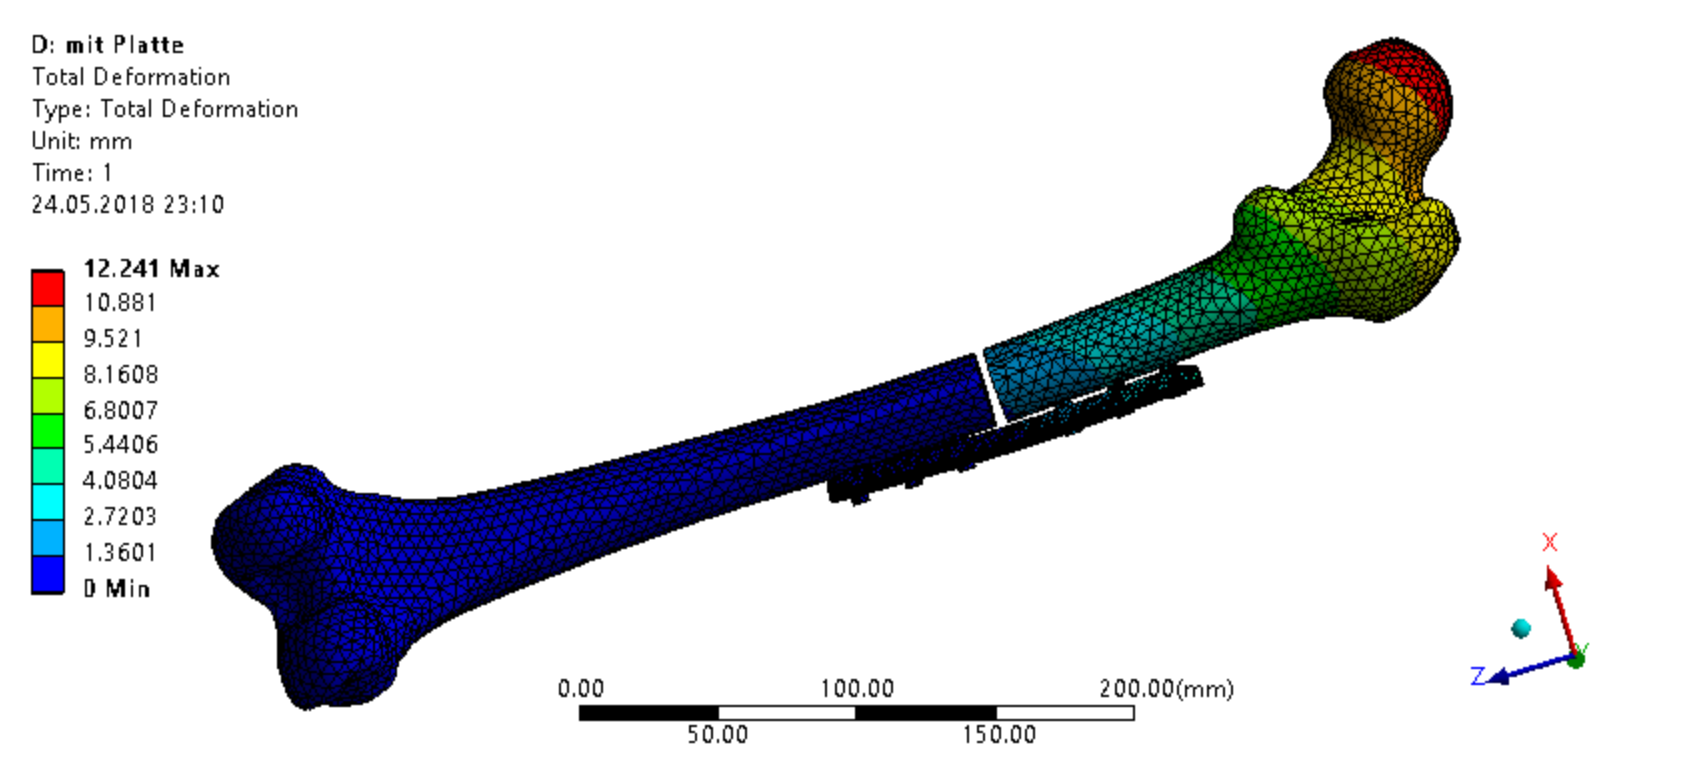
\includegraphics[width=15cm]{content/images/vergleich_deformation.png}
				\captionof{figure}{Gesamtdeformation der Vergleichsplatte}
				\label{fig:vergleich_deformation}
			\end{Figure}
	
	\subsection{Vergleichsspannung}
	
		\begin{Figure}
			\centering
			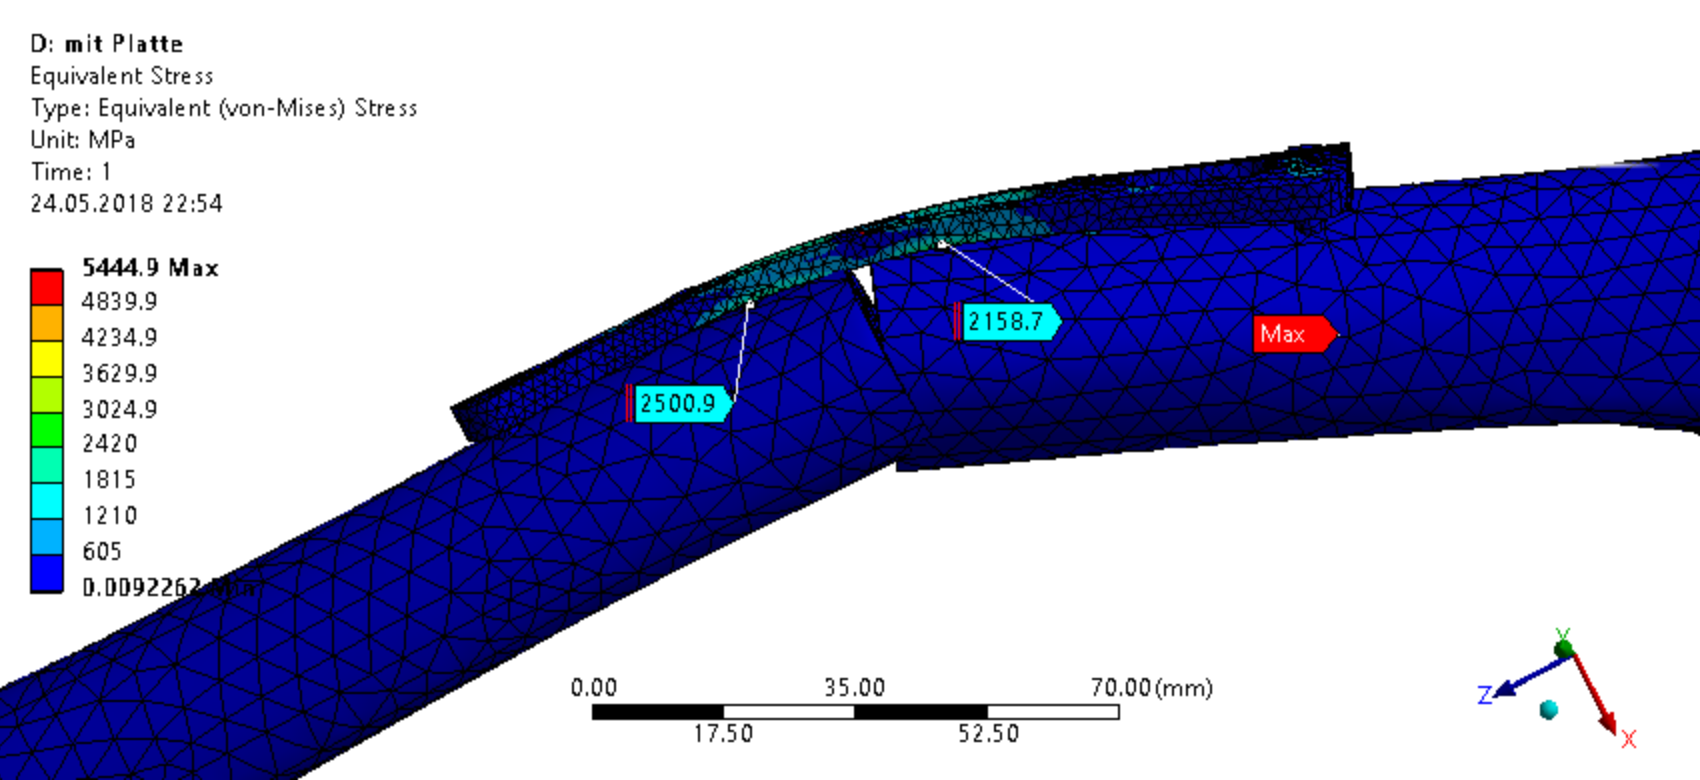
\includegraphics[width=15cm]{content/images/stress_side.png}
			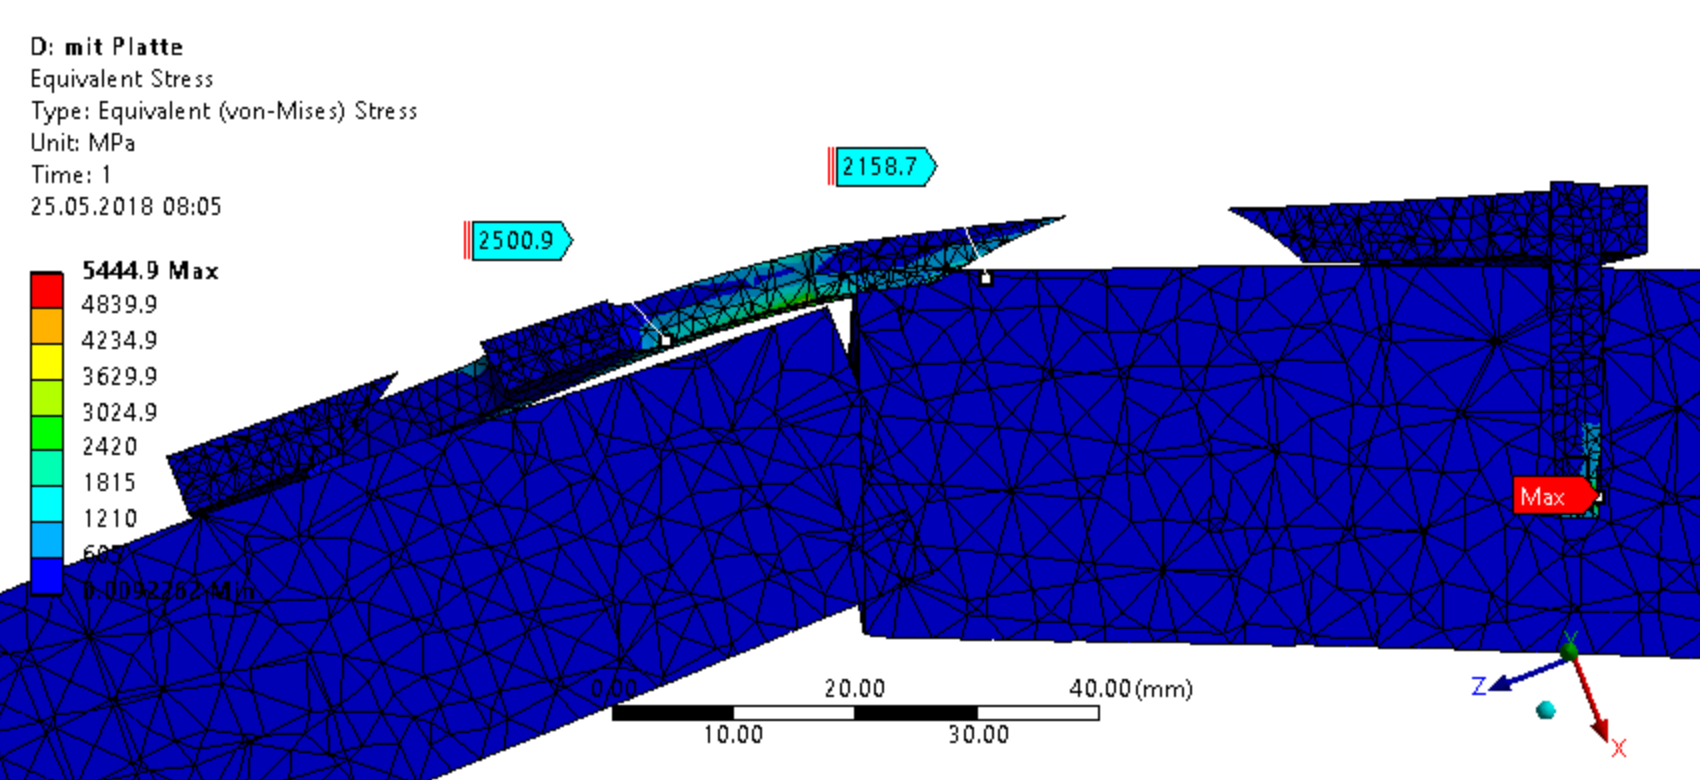
\includegraphics[width=15cm]{content/images/stress_side_profile.png}
			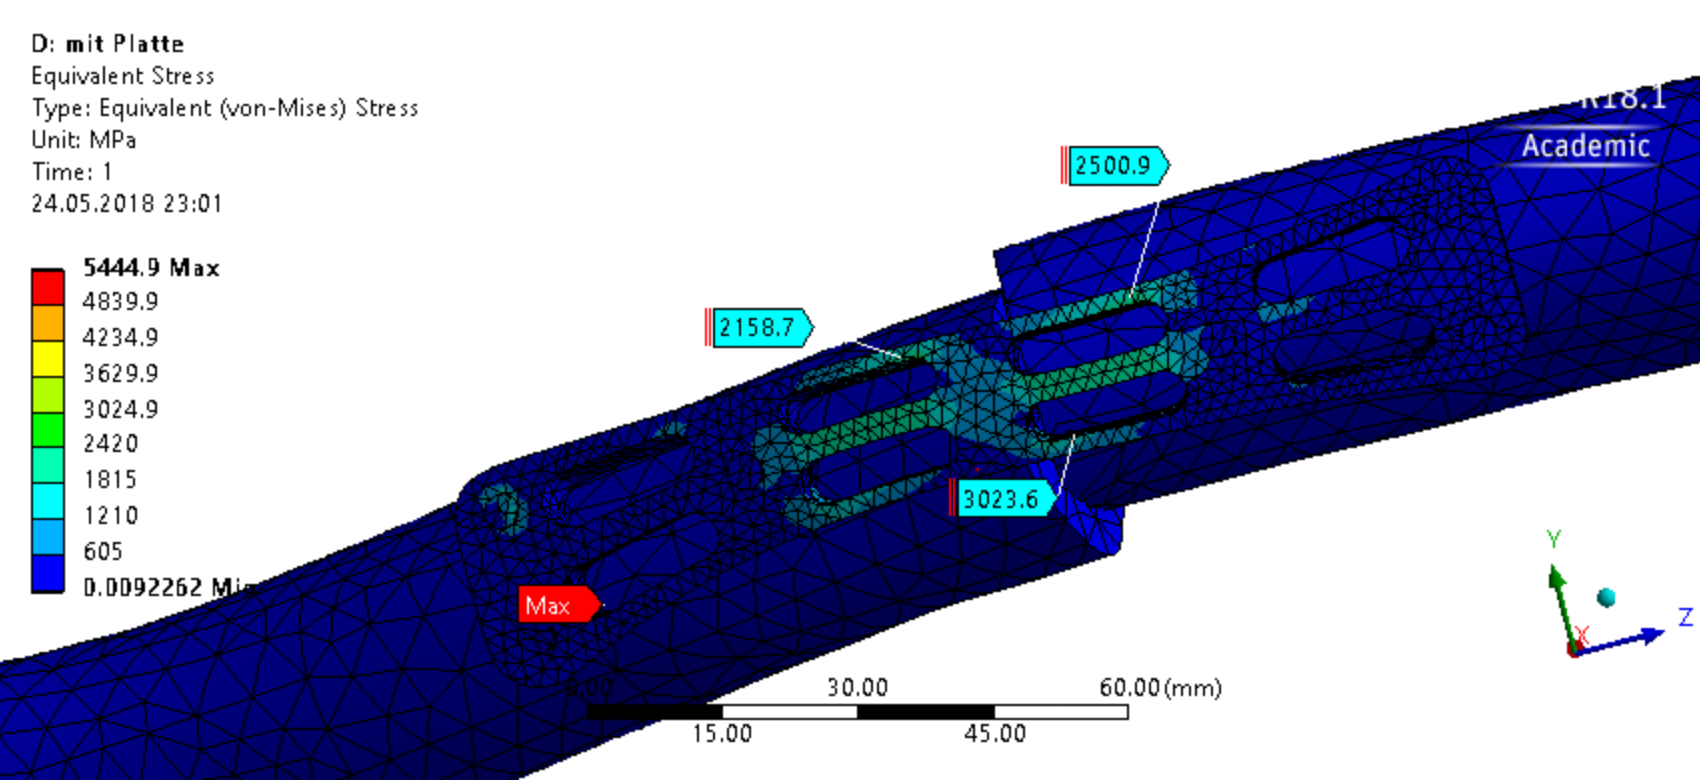
\includegraphics[width=15cm]{content/images/stress_top.png}
			\captionof{figure}{Vergleichsspannung der Osteosyntheseplatte (vorne, Querschnitt, oben)}
			\label{fig:stress_side}
		\end{Figure}
		
		\subsubsection{Vergleichsplatte}
		
			\begin{Figure}
				\centering
				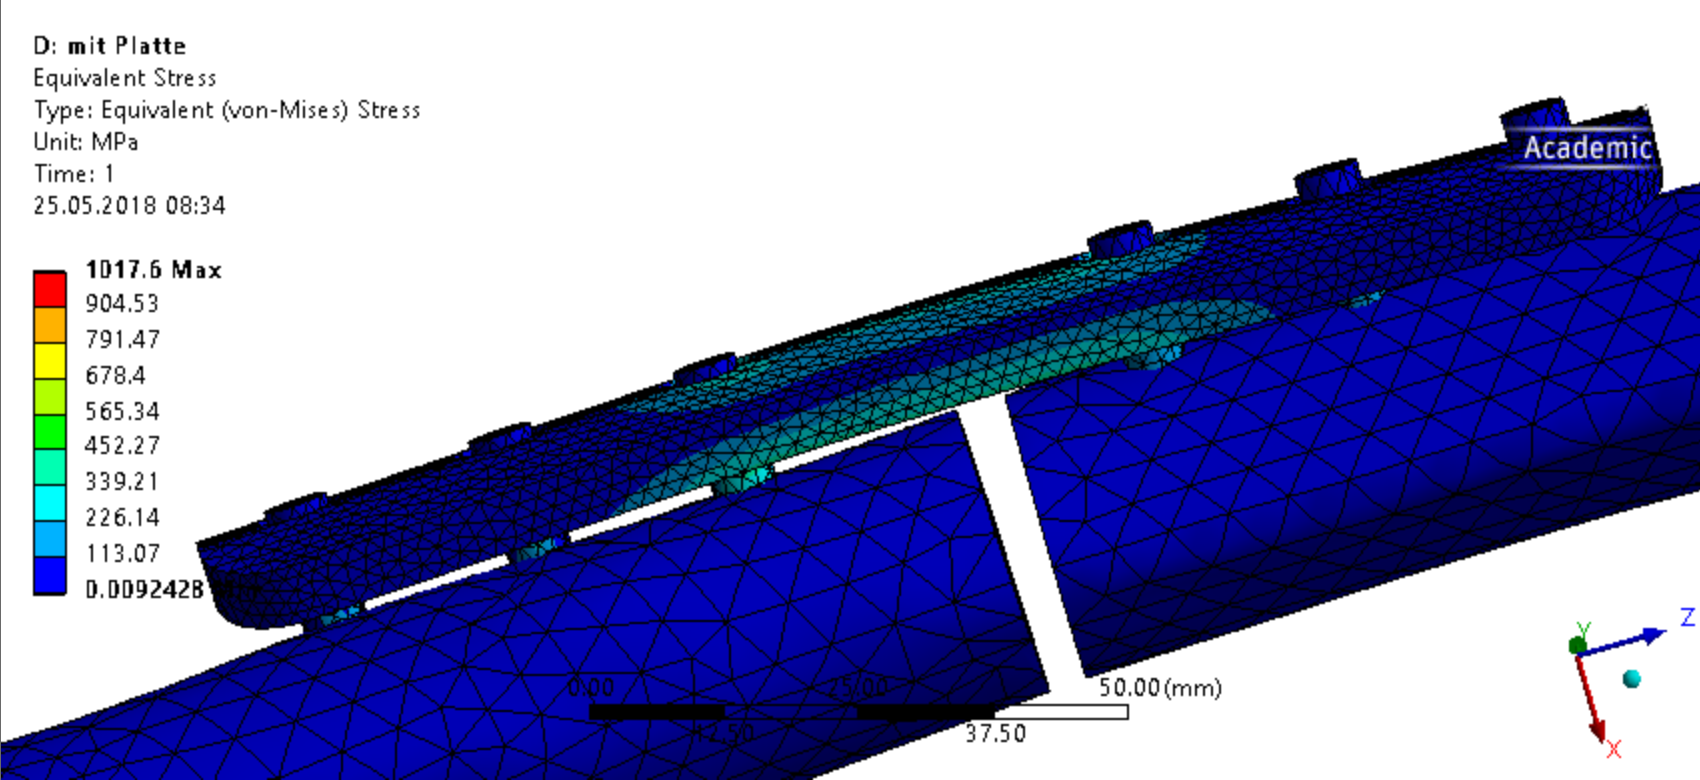
\includegraphics[width=15cm]{content/images/vergleich_stress_side.png}
				\captionof{figure}{Vergleichsspannung der Vergleichsplatte (vorne)}
				\label{fig:vergleich_stress_side}
			\end{Figure}
		
			\begin{Figure}
				\centering
				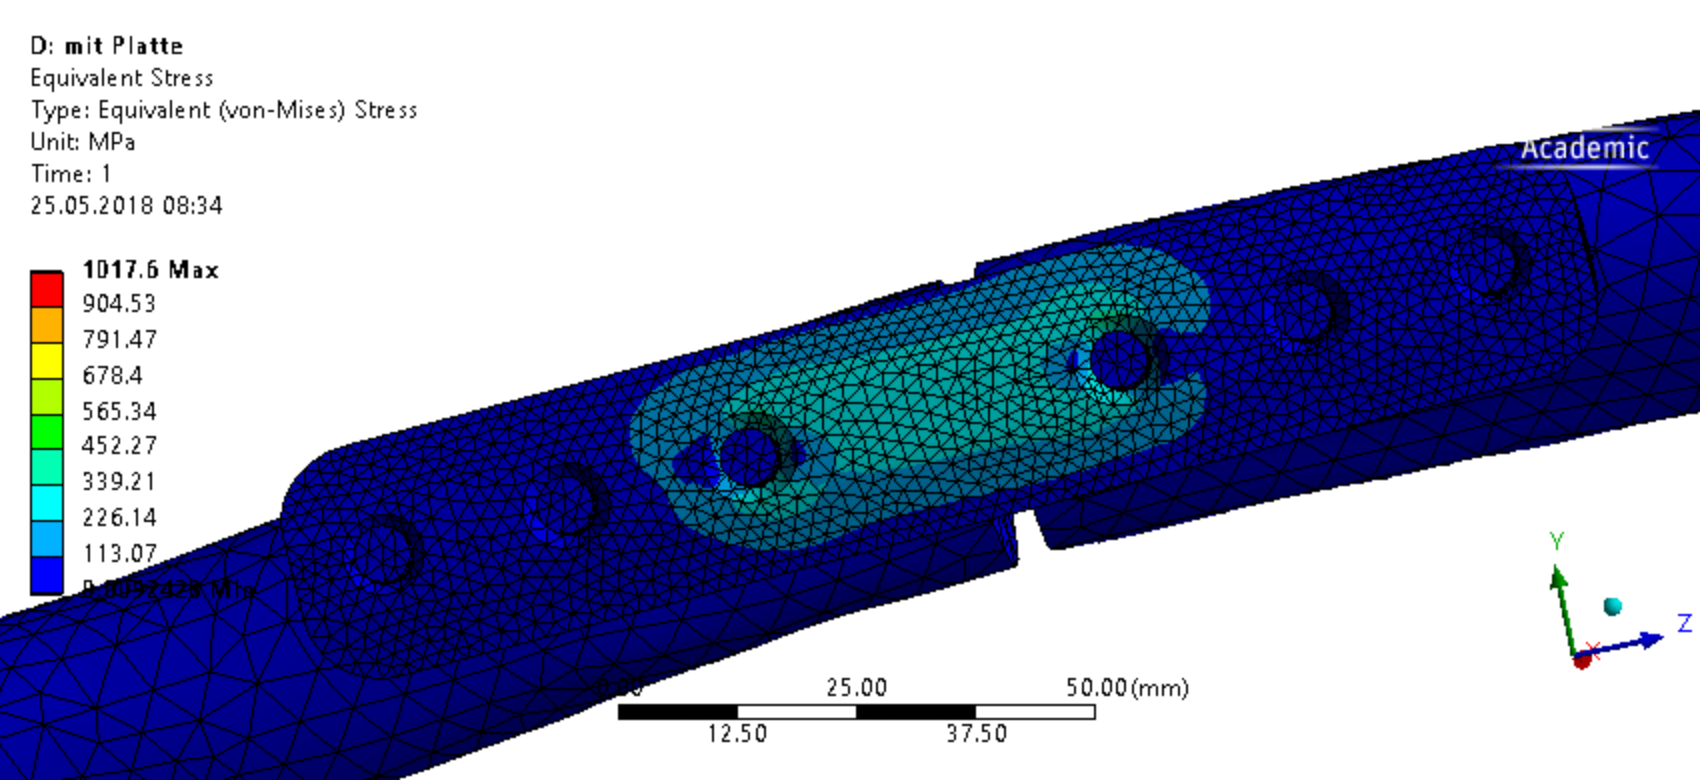
\includegraphics[width=15cm]{content/images/vergleich_stress_top.png}
				\captionof{figure}{Vergleichsspannung der Vergleichsplatte (oben)}
				\label{fig:vergleich_stress_top}
			\end{Figure}
	
	
	\subsection{Gegenüberstellung zwischen den zwei Platten}
	
		Die Gegenüberstellung zwischen der neuen Osteosyntheseplatte und der Vergleichsplatte zeigt,
		dass die neue OSP in der Gesamtdeformation mit $ \SI{88.8}{mm} $ um ein Faktor von $ \SI{7}{} $
		grösser ist	gegenüber der Vergleichsplatte mit $ \SI{12.2}{mm} $.
		
		Auch die Vergleichsspannung der neuen OSP ist mit $ \SI{5444.9}{MPa} $ um ein Faktor von $ \SI{5}{} $
		grösser als die Vergleichsplatte mit $ \SI{1017.6}{MPa} $.
	
	\subsection{Plausibilitätsrechnung}
		Die FE-Simulation soll noch mit einer Plausibilitätsrechnung überprüft werden. Dabei wird der Femur als
		Biegebalken 
		
		Für die Berechnung der Durchbiegung $w\left(l\right)$ wird das Flächenträgheitsmoment $I_{y}$ benötigt.
		Ein Röhrenknochen, wie im gegebenen Fall der Femur, besteht im Querschnitt aus \textit{Compacta},
		\textit{Spongiosa} und einer \textit{Markhöhlen}. Diese haben jeweils einen ganz unterschiedlichen
		Elastizitätsmodul. Zur Abstraktion kann als Durchschnitt ein E-Modul $ E = \SI{17}{GPa} $ und ein
		Flachenträgheitsmoment für einen Kreis wie in Abbildung \ref{fig:moment_of_inertia} benutzt werden.
		
	
		\begin{Figure}
			\centering
			\begin{tikzpicture}
				\node[anchor=south west,inner sep=0] at (-0.5cm,0.5cm) {
					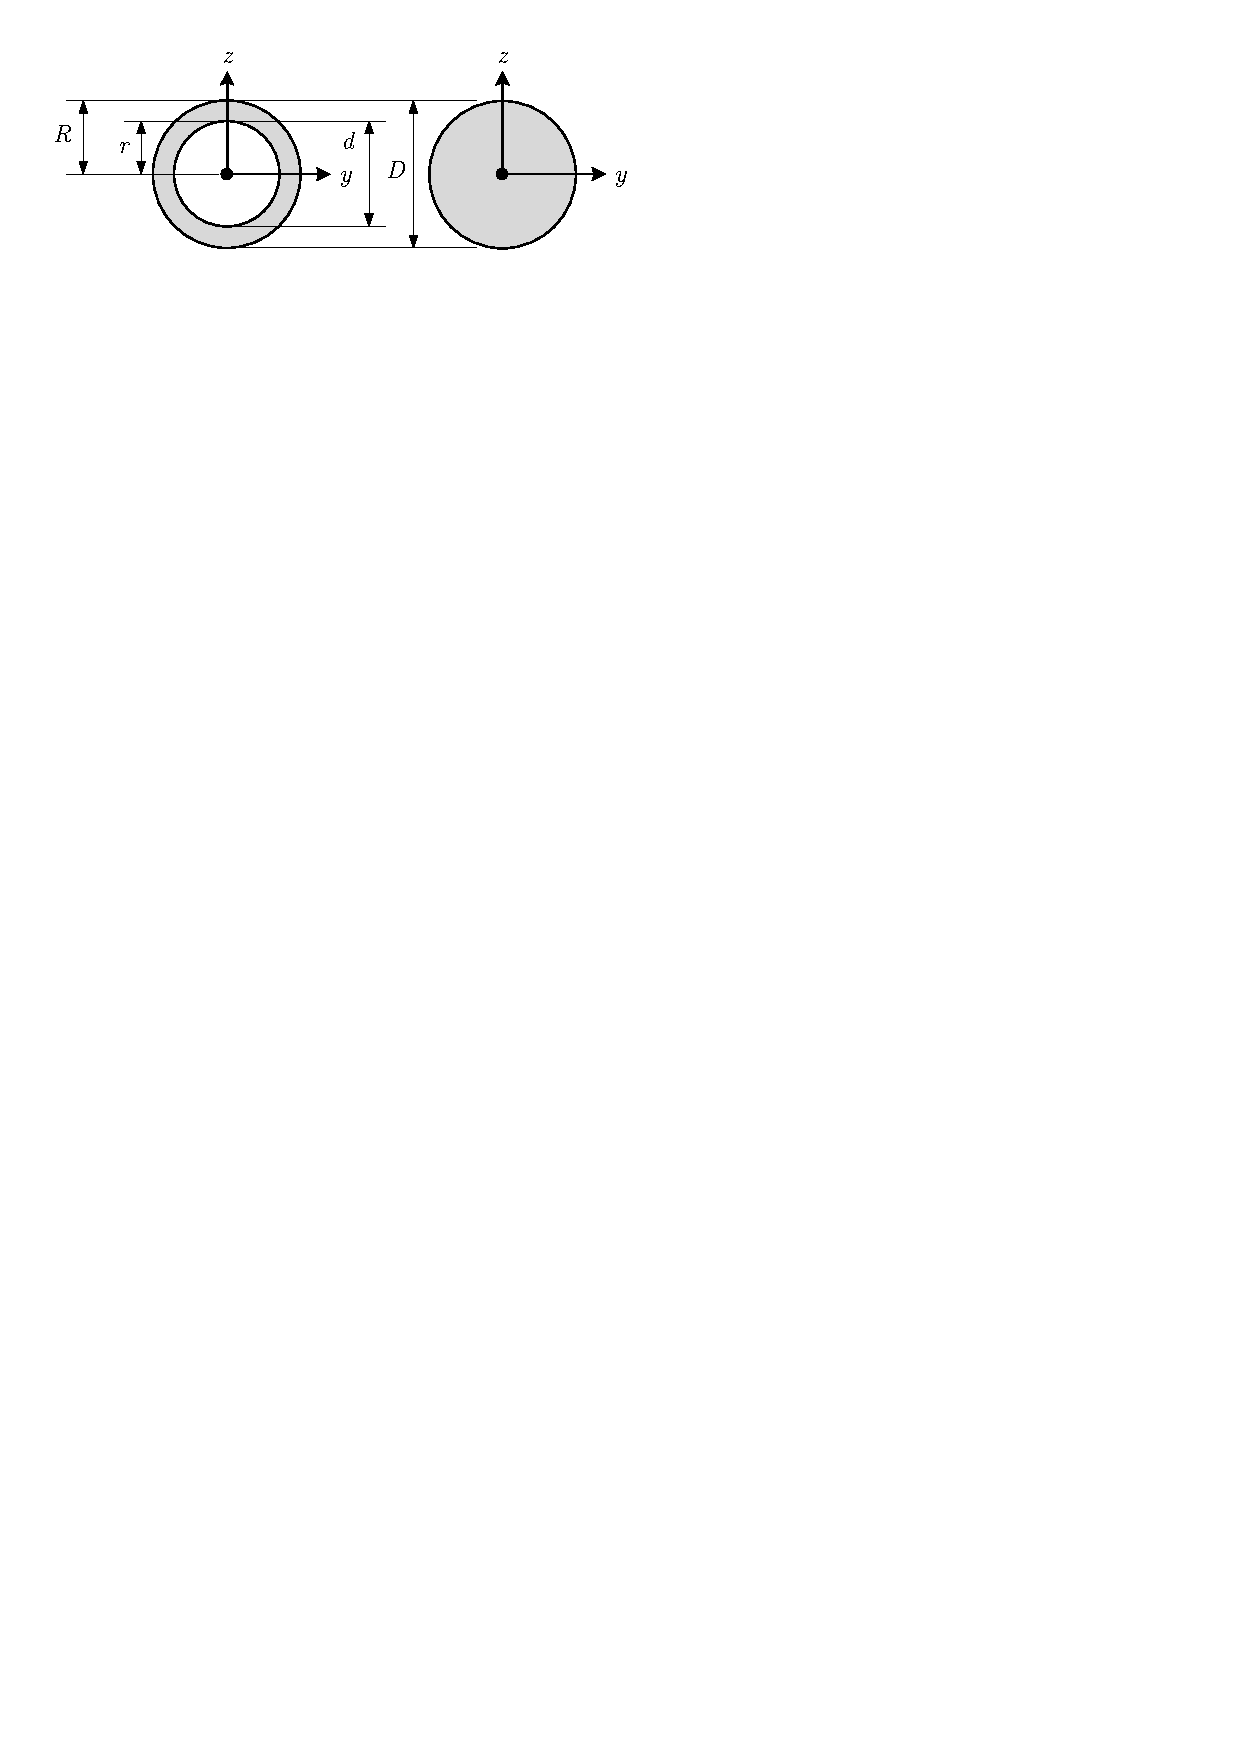
\includegraphics[trim={0.5cm 25cm 10cm 0.5cm},clip,width=10cm]{content/moment_of_inertia.pdf}
				};
				\node (equ1) at (2cm,0cm) {
					\parbox{4cm}{
						\begin{align*}
							I_{y} &= \frac{\pi}{4} \left( R^4 - r^4\right) \\
							      &= \frac{\pi}{64} \left( D^4 - d^4\right)
						\end{align*}
					}
				};
				\node (equ2) at (7cm,0cm) {
					\parbox{4cm}{
						\begin{align*}
							I_{y} &= \frac{\pi}{64} \cdot D^4
						\end{align*}
					}
				};
			\end{tikzpicture}
			\captionof{figure}{Das Flächenträgheitsmoment eines Kreisrings und eines Kreises ($ d = 0 $)}
			\label{fig:moment_of_inertia}
			\vspace*{0.5mm}
		\end{Figure}
	
		\begin{Figure}
			\centering
			\begin{tikzpicture}
			\node[anchor=south west,inner sep=0] at (0cm,0cm) {
				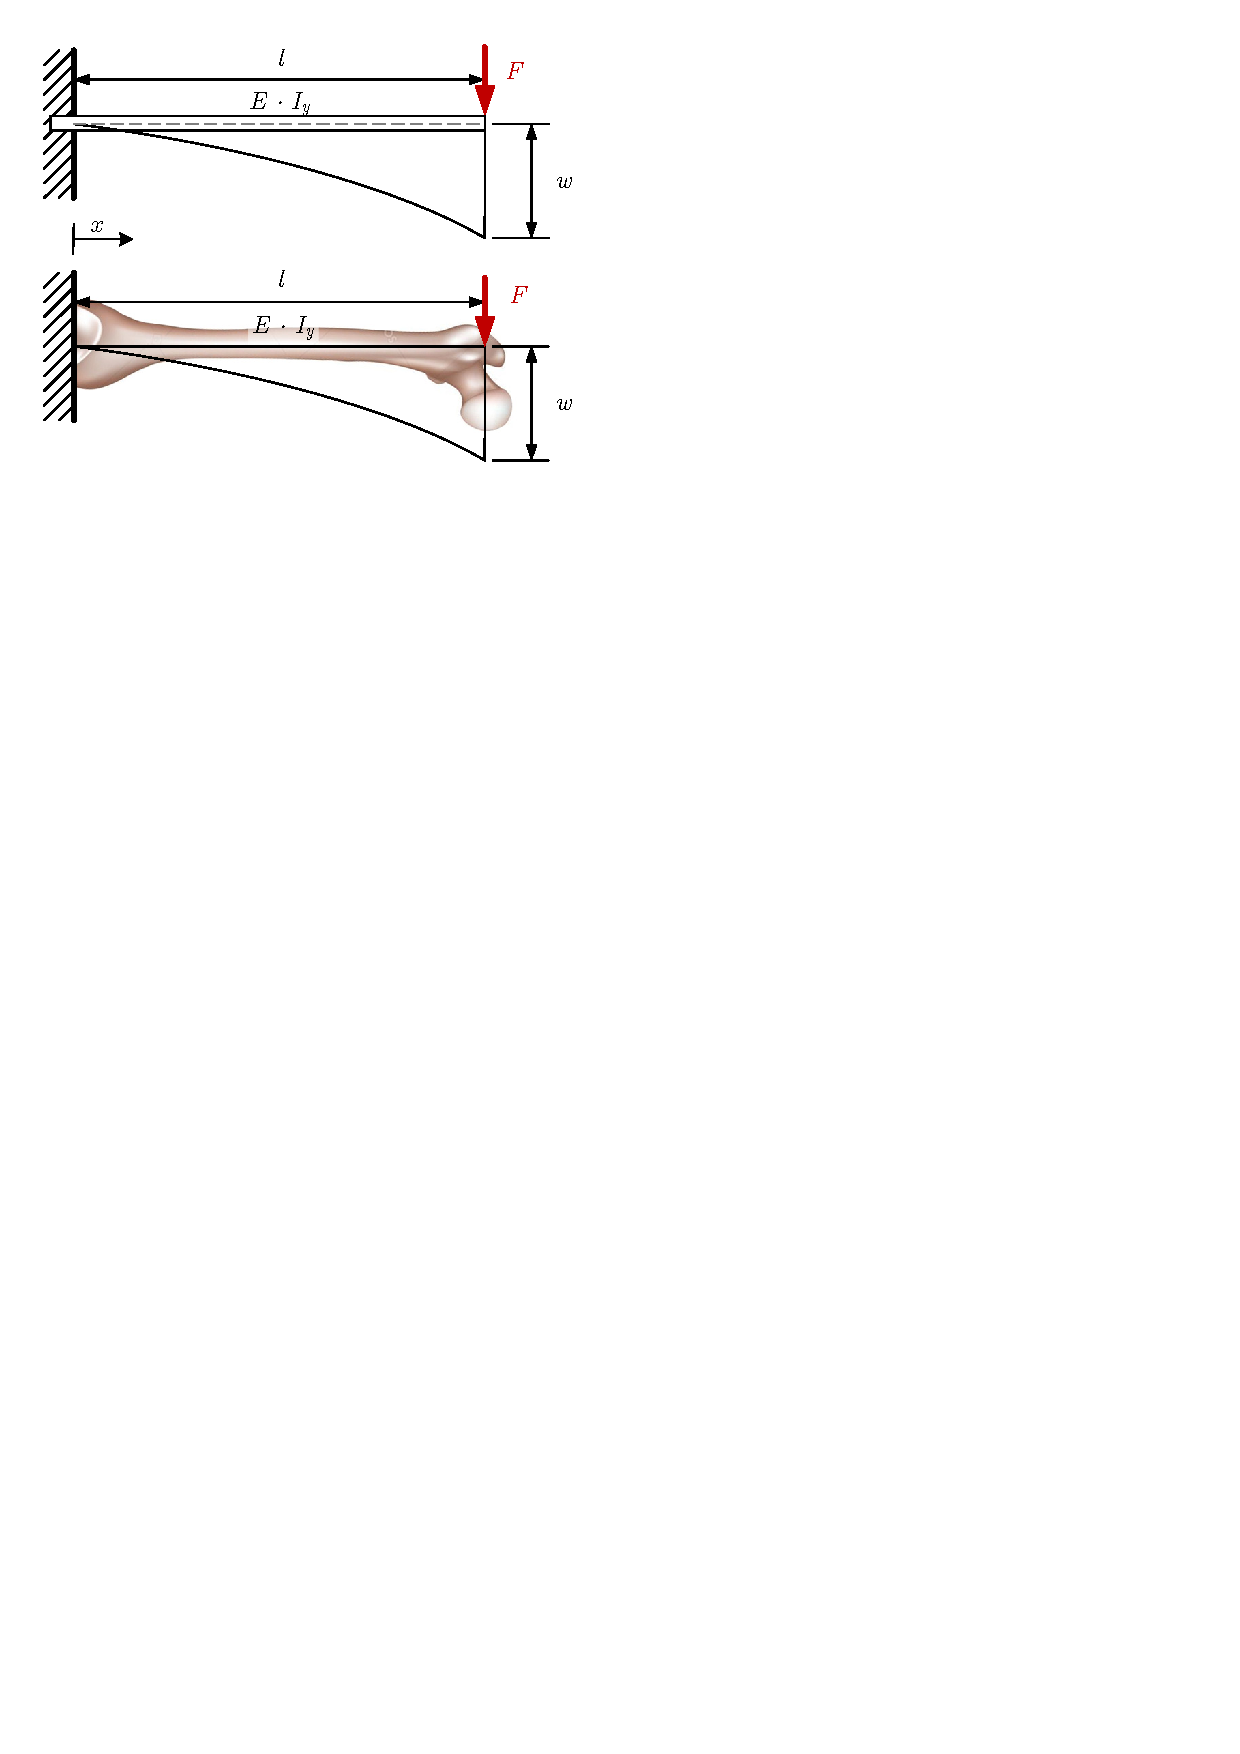
\includegraphics[trim={0.5cm 21cm 11cm 0.5cm},clip,width=10cm]{content/bending_beam.pdf}
			};
			\node (equ1) at (4.25cm,0cm) {
				\parbox{4cm}{
					\begin{align*}
					w\left(l\right) = \frac{F \cdot l^3}{3 \cdot E \cdot I_y}
					\end{align*}
				}
			};
			\end{tikzpicture}
			\captionof{figure}{Die Durchbiegung eines Balkens als Vereinfachung des Femurs}
			\label{fig:bending_beam}
			\vspace*{0.5mm}
		\end{Figure}
	
		Die Berechnung der Verschiebung $w\left(l\right)$ ist in Abbildung \ref{fig:bending_beam} zu finden.
		In Zahlenwerten umgerechnet folgt:

		\begin{mycapequ}[!ht]
			\vspace{-10mm}
			\begin{align*}
				D   &= \SI{30}{mm} = \SI{0.03}{m} \\
				I_y &= \frac{\pi}{64} \cdot D^4 \\
				    &= \frac{\pi}{64} \cdot \left(\SI{0.03}{m}\right)^4 = 3.9761 \cdot 10^{-8} \; \mathrm{m^4} = \SI{39761}{mm^4} \\
				\\
				l   &= \SI{400}{mm} \\
				F   &= \SI{500}{N} \\
				E   &= \SI{17}{GPa} = 17 \cdot 10^{9} \; \mathrm{Pa}
				                    = 17 \cdot 10^{9} \; \mathrm{\frac{N}{m^2}}\\
				w   &= \frac{F \cdot l^3}{3 \cdot E \cdot I_y} \\
				    &= \frac{\SI{500}{N} \cdot \left(\SI{0.4}{m}\right)^3}
				            {3 \cdot 17 \cdot 10^{9} \; \mathrm{\frac{N}{m^2}} \cdot 3.9761 \cdot 10^{-8} \; \mathrm{m^4}}
				     = \SI{0.0158}{m} = \SI{15.8}{mm} \approx \SI{16}{mm}
			\end{align*}
		\end{mycapequ}
	
	
		\subsubsection{Vergleiche der verschiedenen Methoden}
		
			Es wurde der Femur mit OSP in Ansys und der Femur als Biegebalken in einer Handrechnung berechnet.
			Sie können nun in einer weiteren FE-Analyse mit den zwei vorherigen Resultaten gegenübergestellt werden.
			Diese dritte FE-Analyse nur mit dem Femur ist eine Mischrechnung: sie benutzt den beinahe realen Femur,
			doch wurde nur eine Kraft in x-Richtung benutzt, wie bei der Handrechnung.
			
			Diese sind nun in Tabelle \ref{tab:compare} zu sehen.
		
			\begin{center}
				\renewcommand{\arraystretch}{1.5}
				\begin{tabular}{ | p{6cm} | r | r | }
					\multicolumn{1}{l}{\bfseries Methode} &
					\multicolumn{1}{l}{\bfseries Verschiebung} &
					\multicolumn{1}{l}{\bfseries Vergleichsspannung}\\ \hline
					
					FE-Analyse OSP              & \SI{88}{mm} & \SI{5444.9}{MPa} \\ \hline
					FE-Analyse Vergleichsplatte & \SI{12}{mm} & \SI{1017.6}{MPa} \\ \hline
					Handrechnung                & \SI{16}{mm} & - \\ \hline
					FE-Analyse nur mit Femur    & \SI{15}{mm} & - \\ \hline
				\end{tabular}
				\captionof{table}{Vergleich zwischen den Methoden}
				\label{tab:compare}
			\end{center}
			
			
			\begin{Figure}
				\centering
				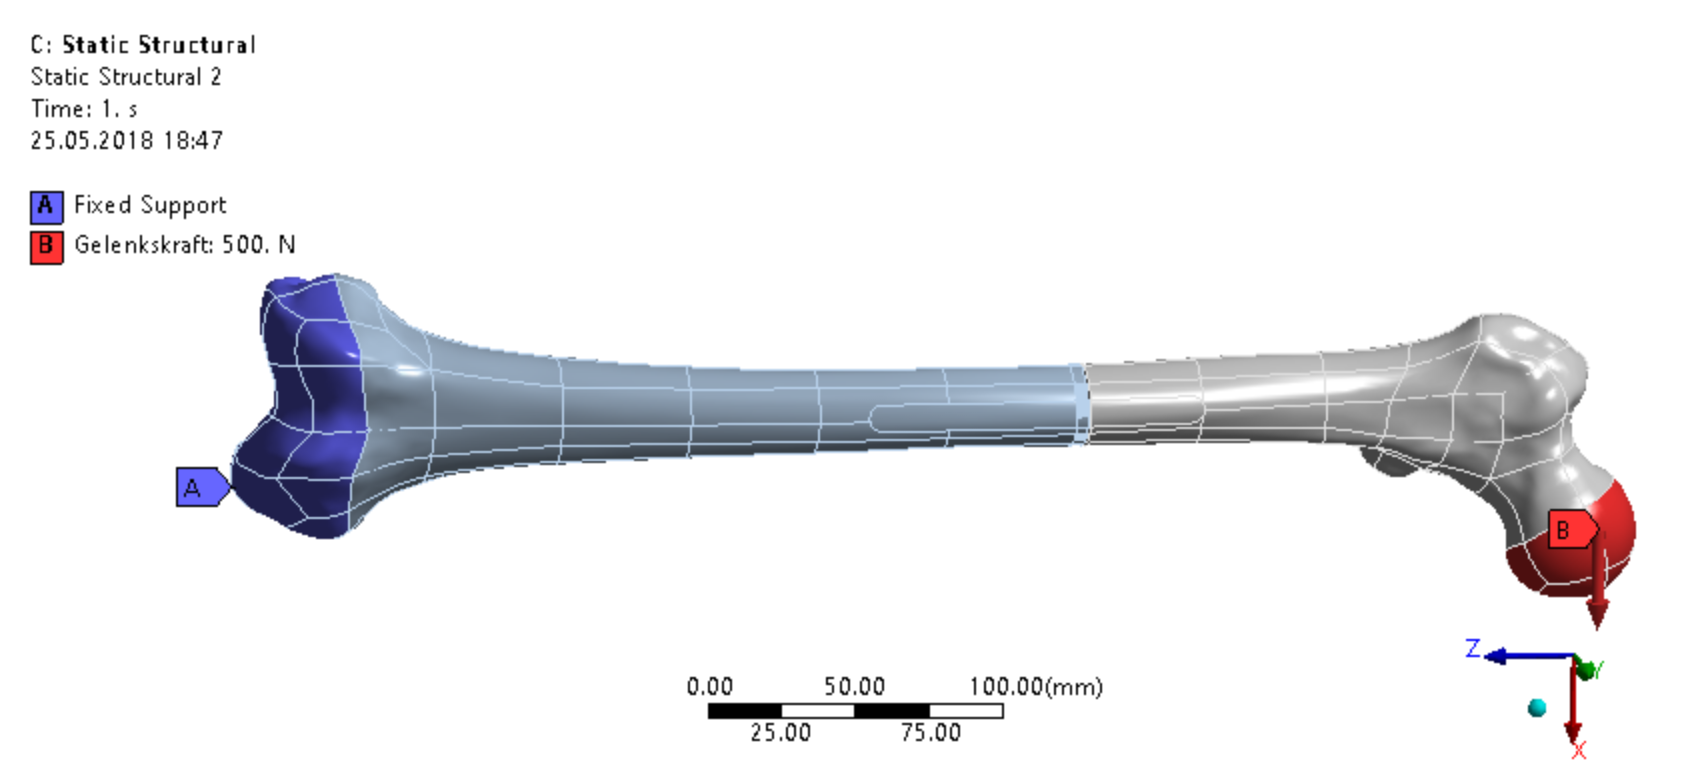
\includegraphics[width=15cm]{content/images/plausibility_forces.png}
				\captionof{figure}{Fest eingespanntes Lager (blau), Kräfte in x-Richtung(rot)}
				\label{fig:plausibility_forces}
			\end{Figure}
			
			\begin{Figure}
				\centering
				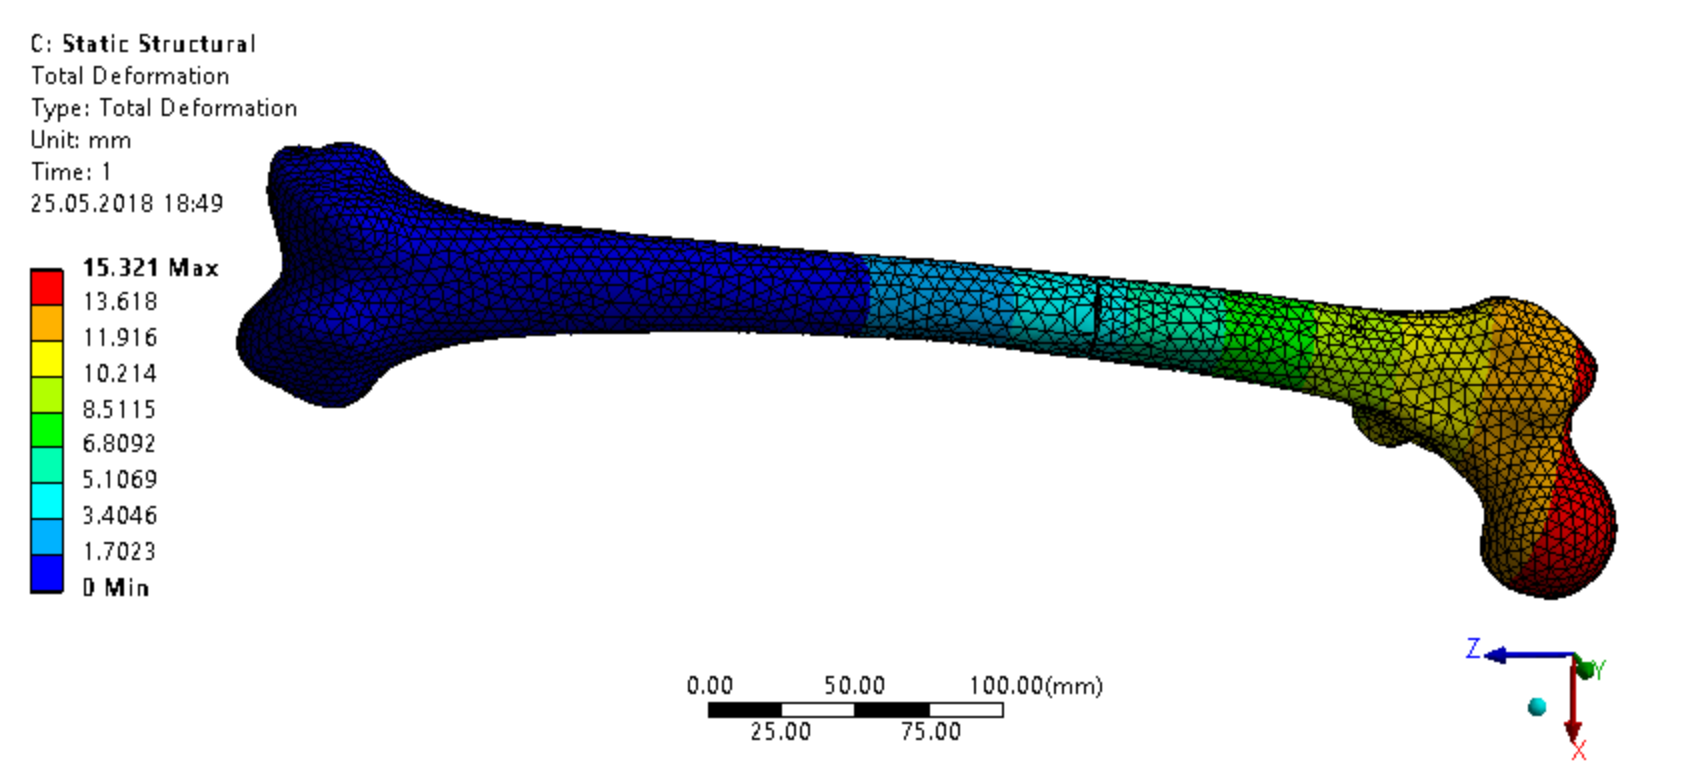
\includegraphics[width=15cm]{content/images/plausibility.png}
				\captionof{figure}{Gesamtdeformation nur mit dem Femur}
				\label{fig:plausibility}
			\end{Figure}

\newpage
\section{Diskussion}

	Die neu entwickelte Osteosyntheseplatte erfüllt die Anforderungen nicht, da die Verschiebung zu gross ist.
	Die Vergleichsplatte erfüllt aber die Anforderungen. In einem weiteren Schritt könnte man die Höhe der OSP
	aufstocken auf die Höhe der Vergleichsplatte. Im Nachhinein ist eine Höhe von \SI{5}{mm} bis \SI{7}{mm}
	nicht realisierbar, da sie die Stabilität beeinträchtigt.
	
	Die physiologische und anatomische Strukturen der neu entwickelten Platte sind so gewählt, dass das
	Periost nicht unter Druck gerät und die Blutversorgung stets gewährleistet ist. Dabei können nur
	winkelstabile Schrauben benutzt werden, die die Platte nicht durch Kompression an den Knochen drückt,
	sondern einen kleinen Abstand zum Knochen gewährt.
	
	Da die FE-Analyse mit einer Titanlegierung getestet wurde, ist eine mögliche Produktion Biokompatibel. 
	
	Die jetztige OSP kann zwar nicht als Implantat benutzt werden. Einen Design-Award könnte es aber dennoch
	gewinnen...
	
	

